% Created by: Adrian Cristea (s1449640)

\documentclass[bsc,frontabs,twoside,singlespacing,parskip,deptreport]{infthesis}

\usepackage[utf8]{inputenc}
\usepackage[T1]{fontenc}
\usepackage[table,xcdraw]{xcolor}
\usepackage{booktabs}
\usepackage{graphicx}
\usepackage{lscape}
\usepackage{tabularx}
\usepackage{amsmath}
\usepackage{listings}
\graphicspath{ {./images/} }

\begin{document}

\title{Mining Reddit to Identify Factors that Describe Prominent Links Between Different Communities}

\author{Adrian Cristea}

\course{Artificial Intelligence and Computer Science}

\project{4th Year Project Report}

\date{\today}

\abstract{
%TODO: Add abstract
Abstract will go here
}

\maketitle

\tableofcontents

% Uncomment the following line to get an
%\pagenumbering{arabic}

\chapter{Introduction}

\section{Social Networks and Reddit}

The internet continues to be one of the biggest achievements in human communications, with continued advances in data transfer and storage ensuring that it has become the de-facto medium for communication and socialisation. The newest annual report published by the International Telecommunication Union (ITU) in 2017 shows that almost half the world's population is now online \cite{ICT2017}. What is even more impressive is that, in developed countries, 94\% of young people aged 15-24 actively use the internet, with mobile broadband connections leading the way in adoption \cite{ICT2017}.

The ubiquitous availability of the medium has created new ways for people to interact with each other: the ability to quickly create new content whenever the opportunity arises, and then share it with a large group of friends, or even anonymously on the web, has meant that there is a vast trove of interesting (and not so interesting) content online, available on-demand. In order to make sense of it all, Social Networks were created which allowed people to create and consume content which is more relevant to them, by joining others with simililar interests.

A new paper published by the Pew Research Centre \cite{pew} shows that a majority of Americans routinely use Social Media Networks, with most accessing it on a daily basis. Websites (and applications) such as Facebook, Youtube, Instagram and Reddit, feature heavily in the lives of people, and have a profound influence on the relations they form with other people, the content they produce and consume, and the opinions they form about the world at large. 

While Facebook, a more traditional type of online social network, is the most accessed such online service on the planet according to Alexa \cite{alexa}, it also seems to have hit a plateau in terms of growth of the number users (about 80\% of the total adult population in the US \cite{pew}), and time spent actively on their platform \cite{pew}, at least in the West. Competitors, such as Instagram (which is owned by Facebook) and Snapchat, have managed to attract a large number of younger users (between the ages of 18 and 24), with many confessing to accessing them multiple times a day. Figure \ref{trends} shows the current trends in online social networks: data is taken from Google Trends, which creates these graphs by showing search interest in online platforms, not as absolute values of their total user numbers. 

These networks are all based on the idea of users creating their own connections by following each others activities intentionally, or by adding "friends". Reddit is, in many ways, different: it is a social news aggregation site which styles itself as \textit{"The Front Page of the Internet"}. People who access it do not have to create an account to view most content available on the website. Furthermore, accounts generally are not linked to the real-life names of the individuals who use them, and, while people are allowed to follow other accounts' activities, the focus is on the content, not on who posted it, and when. 

Since its founding in 2005, and has since become on of the most visited platforms on the web, ranking 5th in the UK and 6th globally \cite{alexa}. Registered users, called \textit{"redditors"}, submit content which can range from articles, photos or text posts, which can then be voted on (up or down) by other users. Such content is usually called a \textit{"post"}, and it has two aspects: the linked content, and the comments associated with it. What is interesting about the comments is that they employ the same voting mechanism as the posts themselved, ensuring a hierarchical view of the discussion taking place on a post: the most \textit{"upvoted"} rise to the top, and the most \textit{"downvoted"} are hidden from view. Both posts and comments have a score attributed to them, called \textit{"karma"}, which represents the difference between the total number of upvotes, and the total number of downvotes. User accounts also have a karma score associated with them, that encompasses the totality of their activity on the platform. In order to allow users to directly support the platform financially, Reddit allows users to gift each other \textit{"Reddit Gold"}, which is a feature reserved for situations in which they'd like to express their satisfaction with high quality content. Gold is displayed prominently on posts and comments, and it signifies that users of the community find them particularly thoughtful and engaging.

Posts are organised into \textit{"subreddits"}, which are user-created boards based around a common topic, such as news, science, technology, politics, and even niche interests such as a specific video game or bonsai trees. If a post garners enough interest (and upvotes), it can then be highlighted on the \textit{"front page"}, which is a constantly updated snapshot of some of the most popular content on Reddit. Most users who have not registered for an account can freely browse the front page (or a subreddit), but not comment or vote.

One other interesting aspect of Reddit is the average time spent on it, compared to other social networks: on average Redditors spend 15:47 minutes a day, as opposed to 11:08 on Facebook, and 6:23 on Twitter, as of April 2018 \cite{alexa}. Due to its nature, Reddit is a platform where content is not only shared, but generated and managed by all of its users, and is a major driver of online communication and information distribution across the globe. With billions of people engaging with this social platform, it is intriguing to uncover the underlying patterns of interaction between users and subreddits.

\subsection{Research Objectives}
In the interest of extending the study of social networking communities to the online space, we would like to explore the character of different social groups present on Reddit by retrieving and analying the large caches of posts and comments which are freely available online. Thus we will explore the factors that best describe prominent links between subreddits, based on the work of Jialun Wun \cite{masters}. It will aim to replicate some of its findings by utilising the same network structure and four different selection criteria (described in chapter \ref{methodology}) to show which are the most important and popular subreddits. We will then to try to find a correlation between these and various other measurements, including the total number of comments in a subreddit, and others given by a linguistic content analysis of the most representative comments.

As such, we pose the following research objectives:

\begin{itemize}
	\item \textit{RO1}: Given the same methodology employed by Wu \cite{masters}, we will try to replicate findings that attempt to find factors which describe the popularity of subreddits.
	\item \textit{RO2}: We will then try to explore other factors which could lead to even better results, given our knowledge of Reddit-specific features (gold, karma scores, controversiality factors, and so on).
	\item \textit{RO3}: Finally, we will attempt to employ modern content and sentiment analysis tools that take into account the context present within conversations on Reddit, in order to further our understanding of prominent links between different subreddits.
\end{itemize}

\subsection{Improvements on previous work}

We attempted to improve upon previous projects by addressing some of their limitations:
\begin{itemize}
	\item instead of only gathering data in a one month period (May 2017) of the top 1000 subreddits (by total number of comments), we have expanded that to include the latest data available in a six month period (July to December 2017) on the top 5000 subreddits. According to the online statistics portal Statista, there were over 1.5 billion unique monthly visitors to Reddit for each month in our selected timeframe \cite{statista}, in which, instead of only getting a brief snapshot of about 80\% of the comments \cite{masters}, we have increased that to just over 95\%. Additionally, we increased the number of custom features that rely on Reddit specific features from 2 to 15, a full list of which can be found in section \ref{features}
	\item In the interest of replicating previous findings, we initially employ the same linguistic content analysis tools used in the previous study. However, one of its limitations is that it ignores the context of comments and treats each subreddit as a bag of words, lacking insight into their structure \cite{masters}. We will use higher level content analysis tools, which provide a more comprehensive evaluation of subreddit comments, as suggested in \cite{lowe2002software}.
\end{itemize}

\section{Report Structure}
The rest of the report is structured as follows:
\begin{itemize}
	\item In Chapter \ref{background} we will discuss some of the research done in the past that has given us a deep understanding of the subject we are trying to discuss. We will initially present some studies which specifically involve Reddit, then give the background that justifies the methodology used in this paper.
	\item Chapter \ref{methodology} will offer an elaborate summary of the tools and methods we employed in order to obtain and analyse the data.
	\item In Chapters \ref{results}, \ref{reddit-features-results}, and \ref{content-analysis-results} we will present the results for the three research objectives posed above, then provide a detailed discussion of them in chapter \ref{discussion}, and some future work that remains to be explored.
	\item Finally, chapter \ref{conclusion} will provide a summary of this paper.
\end{itemize}

\chapter{Literature Review}\label{background}
In this chapter we will introduce the reader to the concepts necessary to understand this paper, along with previous work done in this domain. Initially, studies involving Reddit generally will be presented, with details about mining online communities and social network analysis expanding on them. Then, we will broadly present content and sentiment analysis methods and how they can be used in relation to online social networks.

\section{Previous studies involving Reddit and other similar platforms}\label{previous-studies}

\textit{Computer-mediated communication (CMC)} has been articulated by Susan Herring and is defined as communication that occurs through the use of electronic devices \cite{HerringSusanC2004STtO}. Most CMC research focuses on the social aspects  and patterns of online interaction within computer-mediated formats such as instant messaging, discussion forums, and chat rooms. A study which focused on Reddit revealed the difficulty in getting large datasets which included user information such as gender and age \cite{FinlayS.Craig2014AaGi}. Results indicate that the majority of Redditors fall into the the age group of 12-27, but that people over those ages were more likely to have a higher karma score on their comments. Interestingly, the average female poster, while in the minority in terms of total users, was more likely to have longer comment lengths, but lower overall scores. The number of people who indicated that they were over the age of 36 was only 59, out of a total of 734, however, most of this data is self-reported \cite{FinlayS.Craig2014AaGi}. What is more, while there seemed to be a correlation between age and comment score, there seemed to be little difference in terms of the content posted via links, indicating that age has no bearing on the success of submitted content \cite{FinlayS.Craig2014AaGi}. It is of note that this study might show significantly different results in 2018, due to the vastly increased user base since \cite{alexa} \cite{statista}.

\begin{figure}[hbt]
	\centering
    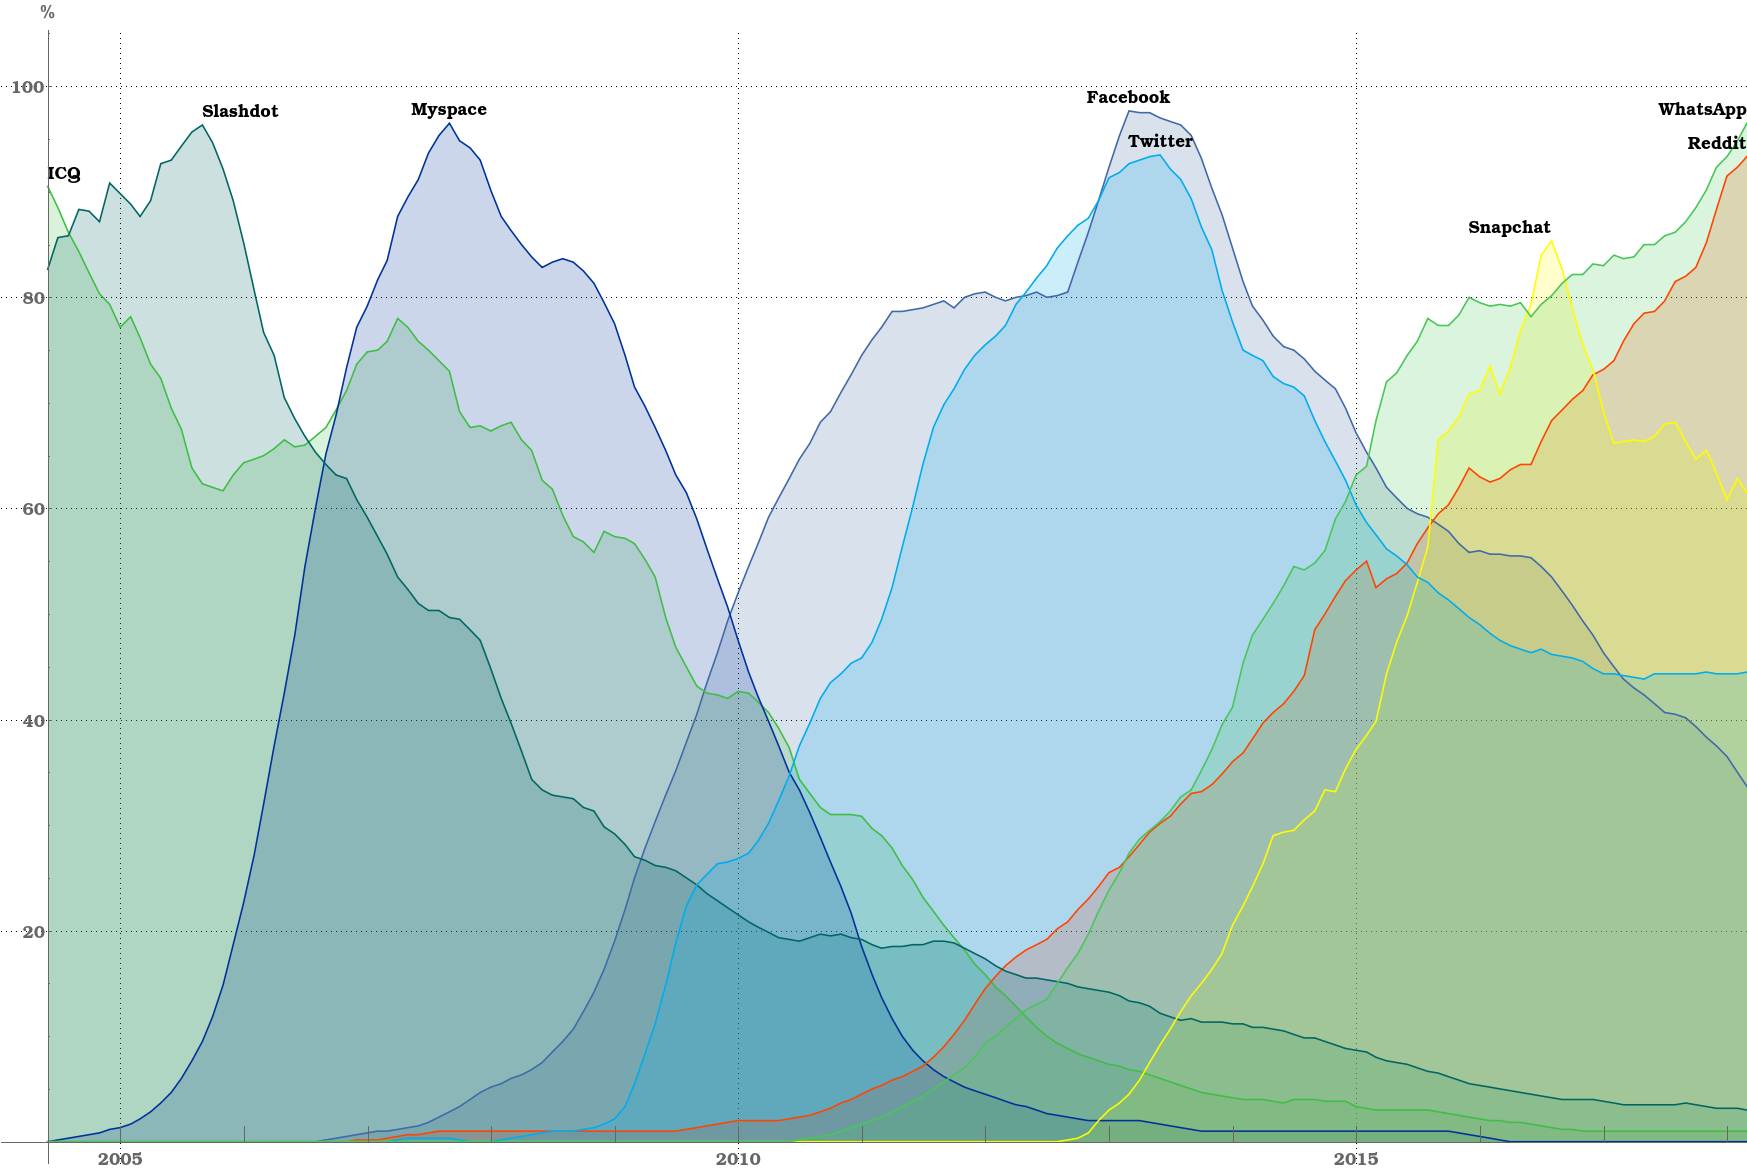
\includegraphics[width=\textwidth]{images/social_networks_over_time}
    \caption{Trends in Social Networks \cite{fig:social_networks}}
    \label{trends}
\end{figure}

Steinbauer \cite{steinbauer} describes Reddit as a social network with user generated content that inherits functionality from social news websites Digg, StumbleUpon and Slashdot. In his paper, he shows that there is a significant gap between the largest subreddits (at the time having a maximum of 1,140,436 of subscribers) and the average subreddit, with only 1077 (in 2012). This provides insight into the idea that a large majority of subreddits are not very active, and this fact can be generalised for the average number of comments on a submission, which seems to be less than 10 \cite{steinbauer}. Furthermore, the way following another user on Reddit works is structured like Twitter, and is not bidirectional as in a classical Online Social Network (the followed user does not get a notification when another adds them as friends, and there is no requirement for them to follow back), which leads to a much looser type of user interaction, on average. 

Lerman \cite{LermanK.2007UPiS} found that in the case of a more tightly connected network, such as Digg, user participation tends to encourage a small number of well-connected individuals to dominate the website. In 2006, the top 3\% of the top 1000 users made 60\% of the submissions that reached the front page. This has lead to the creation of \textit{"voting rings"}, in which large number of connected users voted on each other's posts in order to have a chance of gaining visibility, a type of interaction which is specifically forbidden in Reddit's Terms of Service. It is however impossible to determine whether such interaction still persists, given that there is no way to tell which users added each other as friends using the official API.

The type of topical hierarchy of comments and evolution of a thread of discussion is described by Weninger \cite{WeningerTim2014Aeos}. During the evolution of a thread on a post, new comments are added and users vote on older comments, meaning that as time progresses the average comment depth increases. Furthermore, as the comment depth increases, the discussion diverges significantly from the original topic of the post, and the score of each comment decreases as a function of this this behaviour, and time elapsed since the start. A limitation of this study is that it relied on using the official Reddit API crawler, which restricted access to the data and retrieved only the 100 most popular posts from the 25 biggest subreddits, by number of comment. The way in which our work managed to overcome such limitations is described in section \ref{data}.

To understand the evolution of a content aggregator such as Reddit, Singer et al. \cite{DBLP:journals/corr/SingerFMZS14} released one of the most comprehensive studies at the time, ecompassing all submissions in a period of about 4 years (between 2008 and 2012). It examined the evolution of user comments, and the perception and attention of the community as a whole. One interesting aspect is that they measured the popularity of subreddits by the total number submissions, which should lead to similar results as those which we analysed in our first research question (popularity by total number of comments) in chapter \ref{replication}. They noted the diversification of subreddits, since at the beginning of 2008, the top 20 subreddits accounted for between 70 and 80\% of the total submissions, while at the end of 2012 that number dropped to less than 40\%. Of note is that there has been a large increase in \textit{"self posts"}, which is simply textual content created by the user, as opposed to a link towards an external source, or image. In fact, this type of post has become the largest type of content by total number of submissions, with image posts being the second largest. In our analysis, we found that the biggest subreddit (both by the number of submissions, and comments), by far, is /r/AskReddit, in which users pose a question, and Redditors attempt to answer it. Singer et all. \cite{DBLP:journals/corr/SingerFMZS14} concludes that large online communities with high degrees of freedom can often dramatically change their nature and focus over time, suggesting that \textit{"The Front Page of the Internet"}, might be a more self-referencial, and content generating, community than it's initial direction might have led us to believe.

Another influence on this paper was a study \cite{StoddardGreg2015PaQi} which analysed the popularity of posts on Reddit and Hacker News (a website which shares most of the traits of Reddit, but is focused on a niche of users that are technically inclined). It found that higher quality articles where more popular with the online communities than those of a lower quality, and it evaluated the popularity by the estimated number of user views. We used a similar metric: the total number of comments on a post, which should also be an indication of higher user activity (results described in section \ref{replication}).

\section{Online Communities}\label{online-communities}  
 The concept of an \textit{"online community"} is a natural extension of observed human interaction in the physical world, on the internet. The term was originally coined by \cite{HiltzStarrRoxanne1984Oc:a}, and is a framework that helps make sense of the previously mentioned idea of Computer Mediated Communication (CMC) \cite{HerringSusanC2004STtO}, and the types communities of users that naturally form as a result of their use. The definition seems to have shifted over time, from a \textit{"virtual community members consist of members distant with each other"} \cite{masters}\cite{RheingoldHoward1994Tvc:} to one which seems to describe modern online communities present in social media rigorously \cite{PorterConstanceElise2004AToV}: \\
 
\begin{quotation}
\textbf{\textit{"a virtual community is defined as an aggregation of individuals or business partners who interact around a shared interest, where the interaction is at least partially supported and/or mediated by technology and guided by some protocols or norms"}}
\end{quotation}

A useful concept in understanding the explosive success of online communities is that of \textit{"the third place"}, coined by Ray Oldernburg \cite{oldenburg1999the}, which denotes a realm that is outside the home or work. While his book describes what makes such a third place successful and why they are important for civil society, it has been argued \cite{SoukupCharles2006Ccaa} that CMC Systems, such as chat rooms and social networks, exhibit many of the traits commonly associated with a desirable third place: they are accessible and on neutral ground, conversation is the main activity, they emphasise local community, and they are social levelers. As these properties are often difficult to attain in the physical world, there has been a large shift towards the virtual in past decades.

Therefore, the difficulty is in studying online communities is the scope and diversity of users, data, and interaction patterns. Thus, we will leverage concepts defined in the field of Computer-Supported Cooperative Work (CSCW), initially coined in \cite{1988Ccw:}, and further expanded upon in \cite{WilsonPaul1991CSCW}, in order to create a quantitative analysis of Reddit comments. It is briefly explained by Wilson as the term which combines \textit{"[...] understanding of the way people work in groups with the enabling technologies of computer networking, and associated hardware, software, services and techniques."} In order to analyse patterns of behaviour that people exhibit when contributing to online communities such as Reddit, we will need to consider social network analysis, a method that is fundamental in social science research.

\section{Social Network Analysis}\label{sna}
In the interest of successfully replicating results presented by Jialun Wu \cite{masters}, some of the background which lead to decisions made in the methodology of that paper will be presented here. Social network analysis (SNA) investigates social structures by using graph theory and networks \cite{OtteEvelien2002Snaa}. This has been widely applied to other social media networks, such as Twitter \cite{GrandjeanMartin2016Asna}, and can be used to model collaboration, friendship acquisition, and romantic relationships \cite{abraham2009computational}.

\begin{figure}[htb]\label{graph}
	\centering
 	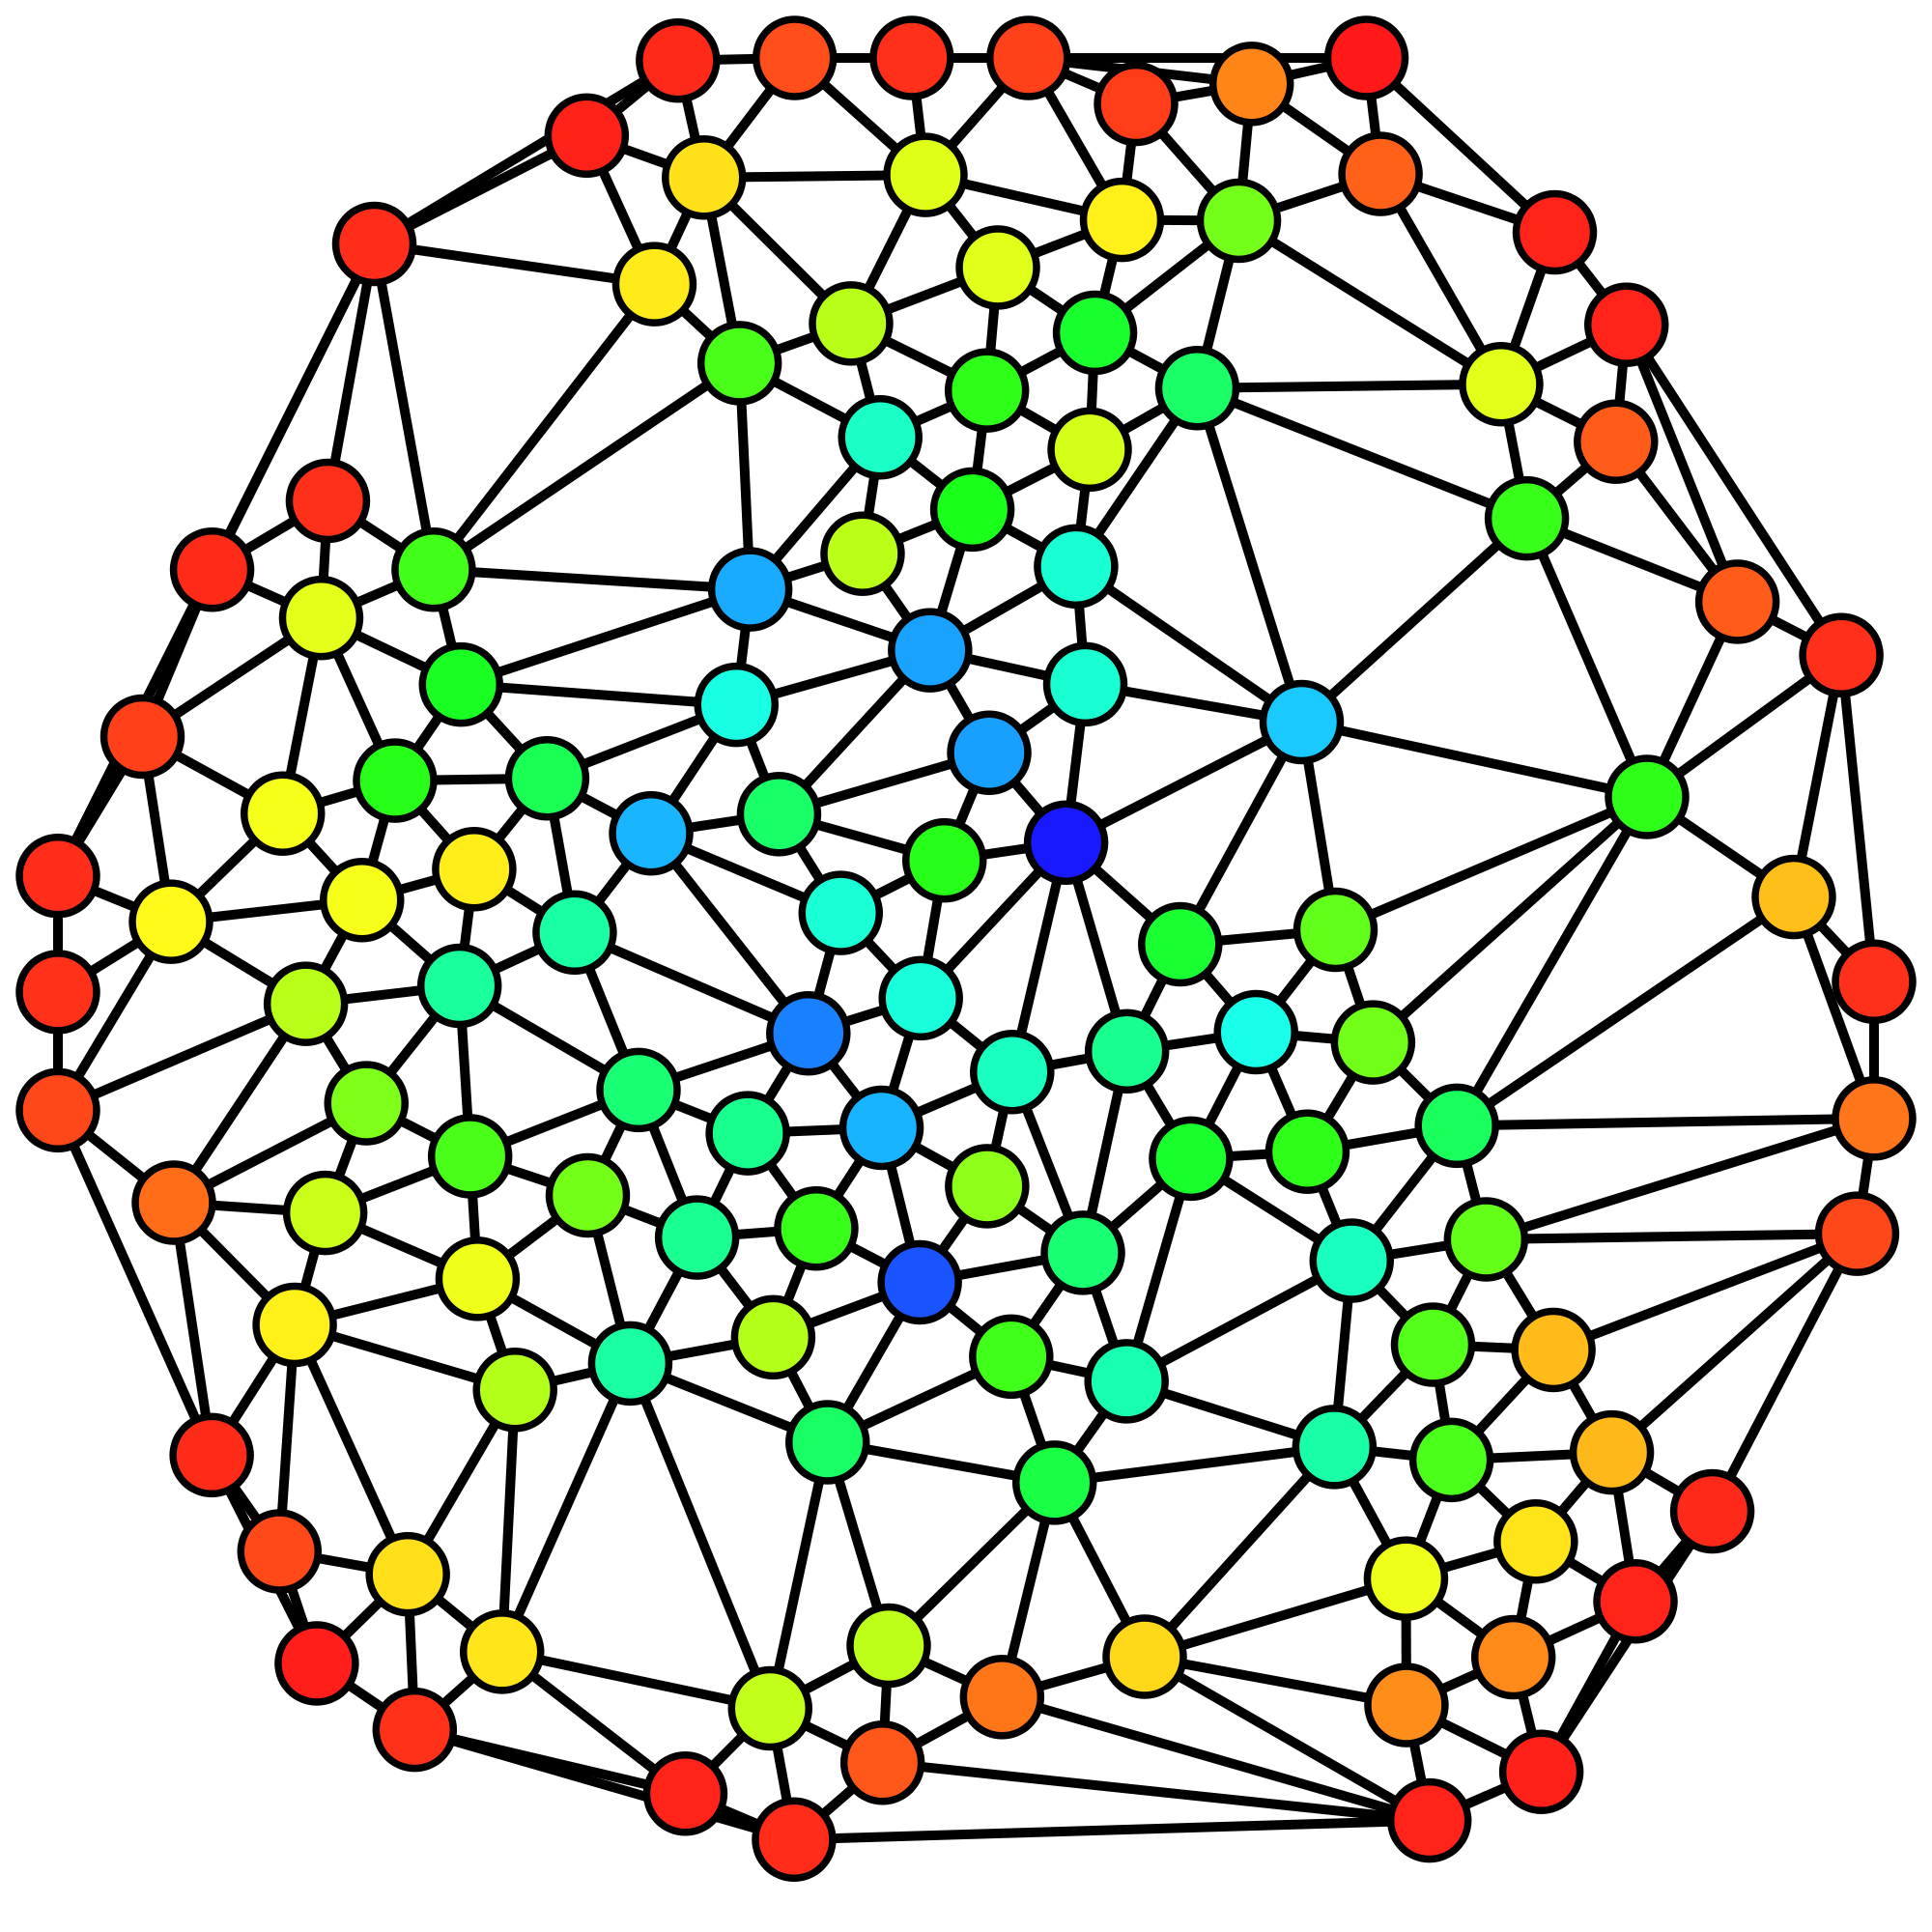
\includegraphics[width=.6\textwidth]{graph.png}
  	\caption{An example of a graph where the hue (from red=0 to blue=max) indicates each node's betweenness centrality. \cite{fig:graph}}
\end{figure}

SNA is applied on network structures characterised by \textit{nodes}, which represent individual people, or distinct things within the network, and \textit{edges}, that determine the relationship between the nodes \cite{OtteEvelien2002Snaa}. This structure is very versatile, and can be used to represent a large number of scenarios, including road maps where the cities are nodes and the roads are edges \cite{masters}. In the case of an online social network as complex as Reddit, serveral options could be viable, including assigning individual users, posts or subreddits as nodes, and their friendship, similarity (by some measure), or concurrent use as edges. In one study that tried to map the "digital humanities community" on Twitter \cite{GrandjeanMartin2016Asna}, it identified the relevant users by use of CSCW (i.e., picking out relevant users from a computer generated pool by hand, and adding relevant data), and assigned edges according to the follower connections the users had with each other. 

Once this structure was created, the authors used \textit{"centrality analysis"} to determine the significance of each node, then clustered users into disctinct language speaker communities (e.g., English, French, Spanish etc.) without ever performing a linguistic analysis of the content. Centrality measurements offer indications that a node has significant connections with other nodes \cite{deLaat2007} \cite{liu2011web}, and are applied to describe each node in the whole network (by measuring aspects of their edges).

There is no single way to define the importance of a node, and each variant of centrality measurements takes different aspects into account \cite{WassermanStanley1994Sna:}:

\begin{itemize}
  \item \textit{Degree centrality} is probably the easiest to understand from a conceptual point of view: it is simply defined as the total number of links  for each node in the graph \cite{erdos}. 
  \item \textit{Closeness centrality} represents the average length of the shortest path between the node and all other nodes in the graph. The more central a node, the closer it is to all other nodes \cite{BavelasAlex1950CPiT}.
  \item \textit{Betweenness centrality} quantifies the number of times a node acts as a bridge along the shortest path between two other nodes \cite{freeman}.
  \item \textit{Eigenvector centrality} assigns a relative score to all nodes on the network, based on the idea that a connection to another high-scoring node is more influential, than one to a lower scoring node. As such, a node with a high score is connected to many other nodes who themselves have high scores \cite{LangvilleAmyN2006Gpab}.
\end{itemize}

An example of an application of the eigenvector centrality in the field of networking is that of Google Pagerank's algorithm, which is based on a variant of the measure we proposed above \cite{pagerank}. It assigns a weight based on the relative importance of each link that is indexed in a set of documents. In the study of sociology, it was found centrality measures, combined with hierarchical clustering, were effective in showing which students were prominent within their social networks, and correlated with other factors such as academic competence, aggression, and popularity \cite{xie1999social}.

\section{Linguistic Content Analysis}\label{linguistic-content-analysis}
We will try to find prominent links between subreddits by measuring some of their aspects quantitatively, namely the number of comments in each subreddit, the average number of posts and authors per day, and so on. However, in order to gain insight into the content of these comments, we will have to rely on \textit{"content analysis"} methods. It is used in social science to quantify patterns in communication, in a replicable and systematic manner \cite{BrymanAlan2015Brm}. Content analysis methods have been used in the past on Reddit, but often relied in developing methods of classification by hand to identify eating disorders \cite{sowlesShainaJ.2018Acao}, or employed basic computerised systems that looked at the size and sharing of messages in order to determine possible interests and benefits to senior citizens \cite{nimrodGalit2010SOCA}. 

We will generate statistical features from selected comments in subreddits in order to quantify their properties from linguistic data. A recent study has been done using these measurements to determine whether there are significant mood changes in the long term present in the population given some circumstances \cite{ethayarajhKawin2017TEoP}. The basic content analysis was implemented using a tool called, \textit{"Linguistic Inquiry and Word Count"} (LIWC), which has been described as dictionary-based content analysis focusing on word count, and basic statistical tests of the raw content \cite{lowe2002software} \cite{masters}. A limitation of this method is that it ignores context, and is unable to distinguish between different word senses \cite{ethayarajhKawin2017TEoP}, although it has been successfully used in the past to measure Post Traumatic Stress Disorder levels on users of Twitter \cite{harman2014measuring}. It offers a feature vector of 98 dimensions for each analysed text, and we will try to see if there is any correlation between these and our centrality results.


\section{Sentiment Analysis, Personality Traits, and Engagement}\label{sentiment-analysis}

We will expand our content analysis tools by the use of more advanced tools which rely on \textit{"sentiment analysis"}. Often regarded as \textit{"opinion mining"}, it is a technique used in natural language processing to systematically derive and quantify subjective information from written text or speech excerpts \cite{sentiment4} \cite{sentiment5}. It aims to extract the attitude of the author or speaker about a specific topic. The two basic tasks of sentiment analysis are emotion recognition and polarity detection \cite{sentiment4}. The former focuses on extracting a set of emotion labels, such as anger, joy or fear, while the latter is a form of binary classification task, defining two opposite emotional states, such as ‘positive’ vs ‘negative’ or ‘good’ vs ‘bad' \cite{sentiment4}. 

Initially developed by Pang and Lee in the early 2000s \cite{sentiment2}, sentiment analysis has been extensively used in fields ranging between finance, marketing and social media analysis, to gain valuable insight about online social communities. 

A study conducted by Keneshloo et al, 2016 \cite{sentiment14}, successfully predicted the popularity of news using sentiment analysis and other language features, highlighting the importance of this text analysis technique. Furthermore, Horne et al. \cite{sentiment3} use sentiment analysis in their study of social signals that influence Reddit comment popularity, showing that sentiment based features are more useful in accurate prediction than other categories. 

According to the Big Five personality model \cite{sentiment6.1} \cite{sentiment6.2}, the five main personality traits can be identified as Openness (to experience), Conscientiousness, Extraversion, Agreeableness and Neuroticism, which can be treated as bipolar items. To illustrate, extraversion can be rated on a range from ‘extraverted, enthusiastic’ to ‘reserved, quiet’.

A study conducted by Selfhout et al. \cite{sentiment7} aimed to identify links between the main five traits and the friendship selection process on social networks. Thus, a reliable model for social network friendship prediction has been built using the respective personality traits. A limitation of the study was that the five personality traits were self reported by the participants in the study. In section \ref{indico} we will use a tool which generates personality trait scores for each of the subreddits. These measurements are generated using a built-in prediction model created with the help of transfer-leaning based machine learning algorithm. For this purpose, we only use only four of the five traits - Openness, Conscientiousness, Extraversion and Agreeableness. 

FA final metric in judging online social network Twitter is that of the \textit{"social engagement"} factor that can be defined as the degree to which one participates in a community \cite{sentiment8}. While it has been usefully applied in the past to rank a set of 264 Universities in the United States by analysing content on their official Twitter accounts, and finding a correlation between the user engagement with them, and their official ranking in a the Times Higher Education, Academic Ranking of World Universities, it has not been used in a significant way to study Reddit. We will attempt to use this concept as a final factor that can help explain the popularity of subreddits.


\chapter{Methodology}\label{methodology}

\section{Overview of the methodology}\label{method-overview}

In this chapter we will offer an overview of the tools and methods employed in the actual implementation of our work. We will initially present the way in which we collected and processed our dataset, the construction of our graph and the subsequent centrality measures applied to it, and finally the way in which we obtained various factors that we used to explain the popularity of subreddits.

\section{Data collection and processing}\label{data}

Since our project requires that we analyze posts and comments on the online social network Reddit, we initially had to gather all the data necessary to run our experiments. There are two ways to do this which don't involve the time consuming task of web scraping: using the official Reddit API, which can be accessed through various API wrappers in different programming languages, and processing, then downloading, a freely available online data dump stored on Google BigQuery with Structured Query Language (SQL) Queries.

\subsection{Official Reddit API}\label{reddit-api}

Reddit provides an official Application Programming Interface (API) which allows users to extract data from the website, including posts, comments, and their associated metadata (their scores, time of creation, number of gold received, and so on), however it limits its usage to a fix number of requests per day. In the past, the size of the data was limited to just a few million comments in total, which made utilising this approach possible \cite{singer}, but recent studies have been limited in their size and scope recently because of it \cite{weninger} \cite{autmanHasan2016Acso}. Due to the massive amount of time required to download even a subset of the data, we chose not to use the API, but to resort to a more advanced approach, described in the next section.

\subsection{Google BigQuery and Google Cloud Storage}\label{bigquery}

Google BigQuery is an online web service which enables working with massive datasets in an interactive manner, by leveraging computing support from Google servers. Once the desired tables were created by using SQL Queries, we stored our data in Comma Separated Values (CSV) files on Google Cloud Storage, then downloaded it to our personal computer.

There is a freely accessible dataset on BigQuery, called \textit{"fh-bigquery:reddit-comments"}, which contains all of the reddit comments from 2005 to 2017 (inclusive). Jialun Wu \cite{masters} analysed comments from May 2017 which is a table containing 79,810,360 comments with metadata, resulting in about 21.6GB of data. Table \ref{big-query} gives an example of the schema used in these tables, with all the associated metadata provided for each comment.

\begin{table}[!b]
\centering
\resizebox{\textwidth}{!}{%
\begin{tabular}{@{}l|cc@{}}
\toprule
Field                     & Type    & Example of data                 \\ \midrule
body                      & STRING  & "I'm so happy this is a thing." \\
score\_hidden             & BOOLEAN & null                            \\
archived                  & BOOLEAN & null                            \\
name                      & STRING  & null                            \\
author                    & STRING  & AeroRespawn                     \\
author\_flair\_text       & STRING  & Celtics                         \\
downs                     & INTEGER & null                            \\
created\_utc              & INTEGER & 1493596801                      \\
subreddit\_id             & STRING  & t5\_2qh1i                       \\
link\_id                  & STRING  & t3\_68dyyl                      \\
parent\_id                & STRING  & t1\_dgxwfwo                     \\
score                     & INTEGER & 132                             \\
retrieved\_on             & INTEGER & 1494514468                      \\
controversiality          & INTEGER & 0                               \\
gilded                    & INTEGER & 5                               \\
id                        & STRING  & dgyruj0                         \\
subreddit                 & STRING  & AskReddit                       \\
ups                       & INTEGER & null                            \\
distinguished             & STRING  & moderator                       \\
author\_flair\_css\_class & STRING  & top\_contributer                \\ \bottomrule
\end{tabular}%
}
\caption{Example of table schema for Google BigQuery dataset}
\label{big-query}
\end{table}

While previous works were able to leverage pre-existing data that contained the top subreddits by total number of comments, we initially had to start our work by recreating this list (in order to have the most up to date information). We chose to analyse the top 5000 subreddits in the period from July to December 2017 (inclusive), which represents a big increase from previous work done in this domain. Once we created the list of top subreddits, we had to extract all the comments and associated metadata for each one individually. Finally, we did some pre-processing work which cleaned the data of comments that were \textit{[removed]} or \textit{[deleted]}, either by users, moderators, or website administrators. The final size of our large combined table was 103GB, and contained a total of 466,164,186 comments, which is a bit over a 5 times increase.

Since we didn't need all of the metadata for our project, we settled on the following fields: 

\begin{enumerate}
  \item body - The content of the comment
  \item subreddit - The name of the subreddit which contains the comment
  \item author - The user who wrote the comment
  \item score - The total score of the comment, after calculating the difference between the number of upvotes and downvotes, we will use this to only select the most relevant comments in each subreddit when doing content analysis
  \item gilded - The total number of Reddit gold received by the comment
  \item controversiality - Whether the Reddit algorithms consider this comment to be of a controversial nature in the community (which is a metric that isn't openly defined by Reddit, however observational data has lead us to assume that comments with large numbers of up and downvotes are classified as such, even if the overall score is positive)
  \item created\_utc - This helps us determine when the comment was created, which we will use to generate statistics, such as the average number of posts (or unique authors, gold, controversial comments, and so on) per day in a given subreddit.
\end{enumerate}

The table below will give a comparison of the scope of this project, and previous data by Wu \cite{masters}.

\begin{table}[!h]
\centering
\resizebox{\textwidth}{!}{%
\begin{tabular}{@{}l|ccc@{}}
              & Number of comments & Number of different users & Size of Data \\ \midrule
Previous Work & 79,810,360         & 2,937,308                 & 21.6 GB      \\
This project  & 466,164,186        & 8,558,522                 & 103 GB       \\ \bottomrule
\end{tabular}%
}
\caption{Statistics generated from the data}
\label{tab:statistics}
\end{table}

\subsection{Data Processing and Social Graph Construction}\label{processing}
In section \ref{sna} of the background, we described how we would build a social network graph where we assigned a node to each subreddit and then created edges between them. A link was built between two subreddits whenever the same user commented in both subreddits, and we increased the weight for each subsequent user. As such, the weight of a link between two nodes represented the total number of users who posted a comment in both subreddits.

Because our project was created in Python, building this graph was one of the most computationally expensive parts of the project. In fact, the script which created it ran for only a few minutes on the old dataset of 1000 subreddits in a one month period, but it increased to a few days when run on our larger dataset, a significant exponential increase. Even so, we improved performance by optimising the script where possible (using more efficient data structures, eliminating useless operations where possible), however the biggest performance enhancement came from compiling our scripts with the use of Cython, a built-in library of Python, which built executable C files from our source. While we tried to create a graph using 15,000, then 10,000 nodes, it quickly became apparent that it was infeasible computationally, and hard to parallelise even given significantly more resources. We settled on 5,000 subreddits because this still represented about 95\% of our dataset ( 	441,820,314 comments out of the total of 466,164,186). Figure \ref{top-commented} shows how abruptly the total number of comments in each subreddit decreases, given that it follows a Power Law distribution. We will discuss this fact in section \ref{replication}.

In creating our graph, we only took the data in the \textit{"author"} and  \textit{"subreddit"} fields. We indexed the nodes and gave them a unique id, then created the links using the process describe above. In order to carefully replicate the work described by Wu \cite{masters}, we only kept the first 90\% of links (ranked by weight), and removed those with weights under 2.

When we started out, we initially recreated these steps for the old data, to make sure that everything was working as expected, and that the results were replicable. Then, we tested a small subset of the new data, to gain some insight and correct any issues that arose. Finally, we used this streamlined workflow for the large dataset, a process that took several few days. Results can be found in section \ref{replication}.

\section{Centrality Measures}\label{centrality}
As described in section \ref{sna}, centrality analysis was used to measure the significance of each node in our graph, in order to determine which subreddits were the most popular. Due to there being no single definition of popularity used in social network analysis, we have chosen four different centrality measurements, that take different aspects of our graph into account: degree centrality, closeness centrality, betweenness centrality and eigenvector centrality. These were measured using the standard formulas below, however we leveraged the igraph library (in the R programming language) which contains tools that help in building graphs and calculating these scores for each node, which will be described in section \ref{igraph}.

\begin{center}
	\begin{figure}[!htb]\label{graph}
		\centering
 		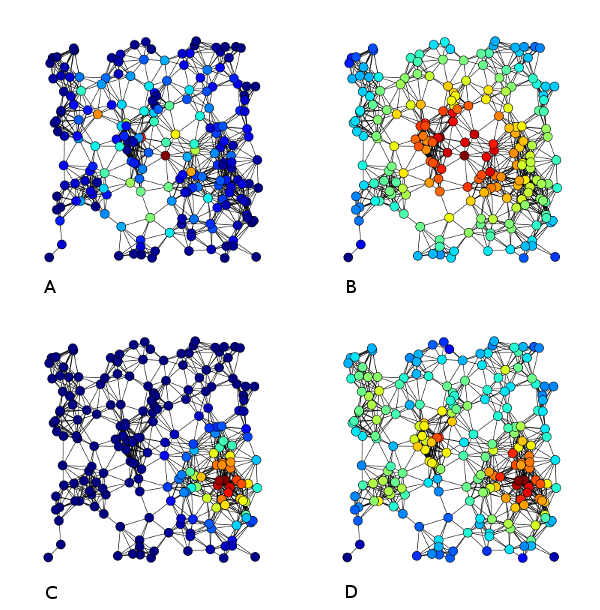
\includegraphics[width=\textwidth]{centrality_measures.png}
  		\caption{Examples of the four centrality measures we have used (A = Betweenness, B = Closeness, C = Eigenvector, D = Degree) (Inverted colours - blue=0, red=max). \cite{fig:centrality-examples}}
  		\label{fig:centrality}
	\end{figure}	
\end{center}

All of the following equations assume a graph $G := ( V , E )$ with $|V|$ number of vertices, and $|E|$ edges.

\subsection{Degree}

Degree centrality is defined as the total number of links for each node in the graph \cite{erdos}. The assumption is that a node which has a large number of connections to others will be a more central and important node, meaning that in our case we simply counted the number of subreddits that were connected to each other. The measurement is given by the following equation:

\begin{equation}
	C_D(v) = \frac{1}{N-1}\deg(v)
\end{equation}

where $C_D(v)$ is the degree centrality of a node $v$, $\deg(v)$ is the number of nodes that link directly to it, and $1/(N-1)$ is the normalisation factor, where $N$ is the total number of nodes in our graph. Figure \ref{fig:centrality} (D) shows an example of such a measurement in a sample graph.

\subsection{Closeness}

Closeness centrality represents the average length of the shortest path between the node and all other nodes in the graph \cite{BavelasAlex1950CPiT}. It is defined as the reciprocal of farness, thus a node with high closeness centrality is one which is able to connect disparate parts of the graph, being closers to all other nodes. The measurement is given by the following equation:

\begin{equation}
	C_C(v)= (N-1)\frac{1}{\sum_x d(x,v)}
\end{equation}

where $C_C(v)$ is the closeness centrality of a node $v$, $d(x,v)$ is the distance between node v and node x, and $(N-1)$ is the normalisation factor, where $N$ is the total number of nodes in our graph. Figure \ref{fig:centrality} (B) shows an example of such a measurement in a sample graph.

\subsection{Betweenness}

Betweenness centrality quantifies the number of times a node acts as a bridge along the shortest path between two other nodes \cite{freeman}. It is usually given as an example in the case of telecomunication networks, where a node with high betweenness centrality would have more information pass through it, thus giving it more control over the network \cite{freeman}, however the argument is easily generalisable to transportation networks as well. The measurement is given by the following equation:

\begin{equation}
	C_B(v) = \frac{(N-1)(N-2)}{2}\sum_{s \neq v \neq t \in V}\frac{\sigma_{st}(v)}{\sigma_{st}}
\end{equation}

where $C_B(v)$ is the betweenness centrality of a node $v$, $\sigma_{st}$ is is the total number of shortest paths from node $s$ to node $t$, and $\sigma_{st}(v)$ is the number of those paths that pass through $v$. As usual, $(N-1)(N-2)/2$ is the normalisation factor where $N$ is the total number of nodes in our graph. Figure \ref{fig:centrality} (A) shows an example of such a measurement in a sample graph.

\subsection{Eigenvector}

Eigenvector centrality assigns a relative score to all nodes on the network, based on the idea that a connection to another high-scoring node is more influential than one to a lower scoring node. As such, a node with a high score is connected to many other nodes who themselves have high scores \cite{LangvilleAmyN2006Gpab}. Let $A = (a_{v,t})$ be the adjacency matrix, i.e. $a_{v,t} = 1$ if vertex $v$ is linked to vertex $t$, and $a_{v,t}=0$ otherwise. Then, 

\begin{equation}
	C_E(x_v) = \frac{1}{\lambda} \sum_{t \in M(v)}x_t = \frac{1}{\lambda} \sum_{t \in G} a_{v,t}x_t
\end{equation}

where $M(v)$ is a set of the neighbors of $v$ and $\lambda$ is a constant. In practice, this value will be normalised over all $N$ nodes. Figure \ref{fig:centrality} (C) shows an example of such a measurement in a sample graph.

\section{Regression and Statistical Analysis}\label{regression-and-stats}

In order to find a correlation between our centrality measurements and the features given by our subreddit properties (described in section \ref{features}), the LIWC analysis (described in section \ref{liwc}), and the indico.io Sentiment Analysis API (described in section \ref{indico}), we created a linear regression model that took into account all of our input features, and added a constat bias factor. The output was given by the four centrality measures, thus we had to run every experiment four times.

In his research, Wu \cite{masters} created two regression models for each experiment: it took all of the input features as predictor variables then ran it for each of the four output variables, and based on these preliminary results, created a second model with a two-step optimising method:

\begin{enumerate}
	\item Evaluate the multicollinearity with the \textit{"variance inflation factor"} (VIF), given that it indicates whether the input feature has a strong linear relationship with another feature \cite{fox}. The predictor with the largest VIF value was removed, and this process was repeated until all VIF values were below 10, a threshold suggested by Myers \cite{myers}
	\item Use a stepwise regression, which is a method for fitting regression models by choosing the predictive variables by an automatic procedure \cite{ralston1960mathematical}. Several ways in which to do this is possible, but Wu \cite{masters} chose the \textit{"Akaike information criterion"} (AIC) as the optimising value, as it is widely used in measuring the fitness of the model \cite{akaike1998information}. Once the AIC value stops decreasing, the model is stopped.
\end{enumerate}

We will present the results for the full array of features in section \ref{regression-all}, then for the stepwise regression in section \ref{regression-stepwise}. As with the regression technique used, we will try to present the same statistical measures by which to judge our results as in previous works:

\begin{itemize}
	\item p-value, also called the asymptotic significance, is the probability that for a given statistical model, the statistical summary would be the same as, or of greater magnitude than, the actual observed results, given that there is no other relationship between the measured phenomena \cite{wasserstein2016asa}.
	\item Multiple R-squared, and Adjusted R-squared, to indicate the percentage of changes in the outcome variables that can be explained by input variables \cite{masters}.
	\item F-ratio, which measures the level of improvement of the prediction of the model compared with the inaccuracy of the model \cite{FieldAndyP2012DsuR}.
\end{itemize}

\section{igraph Package}\label{igraph}
The igraph package (for the R programming language and Python) is freely available for download at: 

\begin{center}
	\begin{verbatim}
		http://igraph.org/
	\end{verbatim}
\end{center} 

It was used in our analysis to conduct the centrality measurements and to fit a linear regression model (described in section \ref{regression-and-stats}), after we used built in functions to create the network model given our nodes and weights, calculated previously. Built-in functions were provided for all of the 4 centrality measurements, quickly speeding up the process of analysing our data.

\section{Subreddit Properties Processing}\label{features}

In section \ref{big-query}, we presented the metadata fields we settled on for each comment in our selected timeframe. We used this information to create factors by using inherent properties of the comments such as the time they were created, the total karma score it received, and whether the Reddit algorithm considered it controversial or not. Some of these have been shown to have a direct link in explaining the popularity of subreddits, to an even larger degree than basic content analysis tools \cite{masters}.

The results of these factors are presented in chapter \ref{reddit-features-results}, but we will summarise our final chosen properties here, with a brief explanation:

\begin{itemize}
	\item AvgAuthor - The average number of unique users that posted in a subreddit, per day. This was a previously used factor by Wu \cite{masters}.
	\item AvgPost - The average number of posts in a subreddit, per day. This was a previously used factor by Wu \cite{masters}.
	\item AvgPostsPerAuthor - The average number of posts created by distinct users for every subreddit
	\item AvgScorePerDay - The average karma that users received in a subreddit, per day
	\item AvgControversiality - The average number of controversial posts in a given subreddit, per day
	\item TotalGold - The total gold received in a subreddit, in the whole timeframe
	\item TotalGoldPerAvgAuthor - The total gold received in a subreddit divided by the number of unique users that posted in it, per day
	\item TotalGoldPerAvgPost - The total gold received in a subreddit divided by the number of distinct posts created in it, per day
	\item AvgGoldPerDay - The average number of gold received in the whole subreddit, per day
	\item AvgGildedPostsPerDay - The average number of gold received per post in a given subreddit, per day
	\item ScoreOver50Count - The total number of comments that had a karma score of over 50
	\item ScoreOver100Count - The total number of comments that had a karma score of over 100
	\item ScoreOver200Count - The total number of comments that had a karma score of over 200
	\item ScoreOver500Count - The total number of comments that had a karma score of over 500
	\item ScoreOver1000Count - The total number of comments that had a karma score of over 1000
	\item ScoreOver2000Count - The total number of comments that had a karma score of over 2000
\end{itemize}

The choice of these measures was given due to our subjective understanding and use of Reddit in the past. Given that the AvgAuthor and AvgPost measures were shown to be an effective measure in describing the popularity of subreddits, we chose to leverage unique features inherent in the functionality of Reddit, that are not available on other online social networks. Results for this part can be found in chapter \ref{reddit-features-results}.

\section{Linguistic Inquiry and Word Count}\label{liwc}

As previously desribed in section \ref{linguistic-content-analysis}, the Linguistic Inquiry and Word Count (LIWC) program has been successfully used in research previously. It was created in the 1990's \cite{liwc}, and has since been used to analyse the content of social networks, including Reddit \cite{ethayarajhKawin2017TEoP}, by using a dictionary based analysis to track the number of occurences of specific words. The latest revision is available online, called LIWC2015. We will use this program to generate a vector of 92 dimensions for each subreddit, by analysing the top voted 500 comments in each of the 5000 subreddits we initially created the centrality measurements for, then run our regression models to find if there is any correlation. Results can be found in sections \ref{regression-all} and \ref{regression-stepwise}.

The latest revision of LIWC, uses a dictionary of 6,400 words, word stems and select emotions \cite{pennebaker2015}. While the system generated vectors of 93 dimensions for every analysed text, they can be largely sorted into the following categories:

\begin{itemize}
	\item \textit{Word Count} - a measure which analyses the total size of the text
	\item \textit{Summary Language Variables} - includes measures for Analytical thinking, clout, authenticity, and emotional tone 
	\item \textit{Linguistic Dimensions} - measures pronouns, articles, prepositions, and so on
	\item \textit{Other Grammar} - counts the number of common verb, adjectives, comparisons, and so on
	\item \textit{Psychological Processes} - counts words which may indicate, positive and negative emotions, social processes such as male and female references, cognitive processes (certainty, insight, etc.), biological processes (health, sexual), drives (achievements, risk, reward), relativity (motion, time, space), personal concerns, and informal language.
\end{itemize}

The justification for analysing only the top 500 comments (by total score) on each subreddit comes from the fact that the LIWC program is very computationally intensive on a personal computer. Given that Wu \cite{masters} did not specify how many were used in his research, we reached this number by trial and error, on the May dataset. Another limitation of LIWC is that it ignores context, and is unable to detect sarcasm or irony \cite{liwc}. To solve both of these issues, we used a more advanced cloud computing tool, described in the next section.

\section{indico.io Sentiment Analysis}\label{indico}

Indico.io is an online RESTful API that allows users to analyse text, image, and other types of comments using a transfer-learning based, pretrained machine learning algorithm \cite{indico}. Because the model is already trained, and the API makes calls to an online server, this reduce our computation time significantly, even though we analysed the same 500 comments, as we did previously with LIWC.

We used four different measures, some of which mirror categories available in LIWC. All of the returned results are probability measures:

\begin{itemize}
	\item \textit{Sentiment Analysis} - Determines whether a text is positive or negative. For example, the text of a 5 star review is positive, while the text of a 1 star review is negative. The API performs with 93\% accuracy on the IMDB dataset \cite{indico}.
	\item \textit{Emotion} - Predicts the emotion expressed by an author in the following categories: anger, joy, fear, sadness, surprise.
	\item \textit{Personality} - Predicts the personality traits of a text's author: extraversion, openness, agreeableness, and conscientiousness. Note that it lacks any measure of neuroticism, which is one of the five big personality traits we mentioned in section \ref{sentiment-analysis}
	\item \textit{"Twitter Engagement"} - A measure which is used to predict audience engagement on Twitter, but which we found useful in our testing even given large texts found on Reddit.
\end{itemize}

The results for these measurements can be found in chapter \ref{content-analysis-results}, and they can be contrasted with the replicated results in chapter \ref{regression-all} and \ref{regression-stepwise}.

\chapter{Research Objective 1: Replication of Previous Work}\label{results}

In this chapter, we will start by presenting our work done in replicating the results given by \cite{masters}. The aim of that project was to determine the relationship between several characteristics of subreddits, such as the total number of comments in a given timeframe or the average number of posts per day, and the popularity of subreddits, which was measured using centrality techniques, as described in \ref{centrality}. We will present our results for the larger dataset in the first research objective.

Based on those findings, we tried to find additional characteristics which could be relevant to Reddit, such as the average number of gold received on a given subreddit each day. The full list, and a description of these features can be found in section \ref{features}, and we will present the results for these in the second research objective. 

Finally, we have tried to use more advanced content analysis tools, as suggested by \cite{lowe2002software}. The features were generated using an online machine-learning based API that specialises in sentiment and content analysis, called \textit{"indico.io"}. For reference, the categories for these features were presented in section \ref{indico}. We aim to contrast these results with previous work, in our final research objective.

For each of these research objectives, we began by running a linear regression model of our full list of features against each of the four centrality measures. We then proceeded to eliminate the predictors with large VIF values, until the ones that remained had values below 10, as described in section \ref{regression-and-stats}. A final stepwise regression model was fitted for the measures, and these results will show which are the most significant factors that can best explain the popularity of subreddits. 

\newpage

\section{Initial subreddit properties analysis}\label{replication}

\begin{figure}[hbt]
	\centering
  	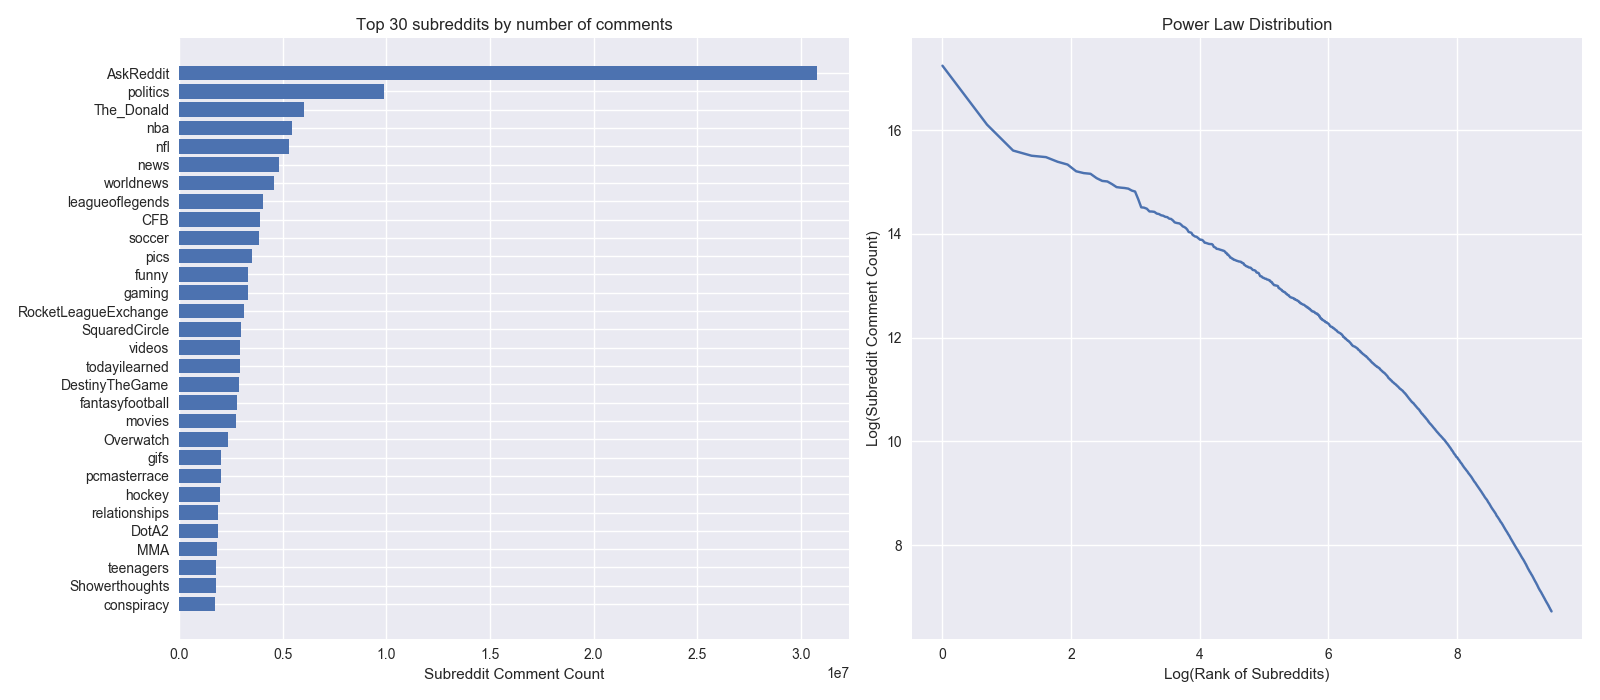
\includegraphics[width=\textwidth]{zipfslaw.png}
  	\caption{Distribution of comments among top subreddits}
  	\label{fig:distribution-of-comments}
\end{figure}

Figure \ref{fig:distribution-of-comments} should offer some perspective on the large gap between subreddits, when taken by the total number of comments. We used this data to construct our social network graph, because we could only analyse a subset of the whole dataset, given computational and time constraints. It roughly corresponds to the Pareto Principle, also known as the 80/20), which states that roughly 80\% of the effects come from 20\% of the causes \cite{pareto}. In our case, we chose to present the distribution of comments counts (for each subreddit) and the relative positions they have with each other by rank, in a log-log scale to show the proportional relationship between the two values. \textit{"AskReddit"}, which the community with the most comments, only allows question-based text-posts, and it has over 30,000,000 comments, while the second largest subreddit, \textit{"politics"}, has less than half that amount.

In order to provide a reference for the centrality measures we obtained below, this table will show the ten most commented subreddits in the last 6 months of 2017. 

\vfill

\begin{table}[!h]
\centering
\resizebox{.6\textwidth}{!}{%
\begin{tabular}{@{}c|cc@{}}
\toprule
\textbf{Rank} & \textbf{Subreddit} & \textbf{Total Number of Comments} \\ \midrule
1 & AskReddit & 30,787,687 \\
2 & politics & 9,885,668 \\
3 & The\_Donald & 5,999,631 \\
4 & nba & 5,428,135 \\
5 & nfl & 5,285,251 \\
6 & news & 4,831,723 \\
7 & worldnews & 4,579,878 \\
8 & leagueoflegends & 4,022,852 \\
9 & CFB & 3,884,399 \\
10 & soccer & 3,832,341 \\ \bottomrule
\end{tabular}%
}
\caption{Top 10 subreddits with the highest number of comments between July and December 2017 (inclusive)}
\label{top-commented}
\end{table}


\newpage

\subsection{Centrality Results and number of comments}

This section will initially show results for the four centrality results compared to the total number of comments in a subreddit. However, we used these same results in all of our subsequent comparisons.

\subsubsection{Degree}

Since the degree centrality measurement is simply defined as the total number of links for each node in the graph, we expected to find large values for these,  as similar results were found in previous studies \cite{steinbauer}. It seems that the the biggest subreddits are very interconnected, leading us to make the assumption that most users frequently interact with many different subreddits. The observed p-value is 0.001, with the R-squared value for degree centrality is being quite low, 0.035, which leads us to conclude that comment count is a significant predictor which doesn't fully explain the popularity distribution, as previously found by \cite{masters}. Of note is that all of the presented subreddits by \cite{masters} appear in the top 10 of our results, but not in the top 5, as were shown previously. Because of this, we decided to include larger tables, to show relative changes in results. Please refer to figure \ref{fig:degree}.

\begin{table}[!h]
\centering
\resizebox{.4\textheight}{!}{%
\begin{tabular}{@{}c|ccc@{}}
\toprule
\textbf{Rank} & \textbf{Subreddit} & \textbf{Degree} & \textbf{Comments} \\ \midrule
1 & AskReddit & 4,988 & 30,787,687 \\
2 & mildlyinteresting & 4,984 & 1,390,705 \\
3 & Showerthoughts & 4,983 & 1,764,335 \\
4 & funny & 4,983 & 3,341,450 \\
5 & pics & 4,983 & 3,522,976 \\
6 & movies & 4,982 & 2,721,654 \\
7 & OldSchoolCool & 4,981 & 705,974 \\
8 & todayilearned & 4,980 & 2,913,802 \\
9 & worldnews & 4,979 & 4,579,878 \\
10 & videos & 4,979 & 2,934,422 \\ \bottomrule
\end{tabular}%
}
\caption{Top 10 subreddits ordered by their degree score}
\label{top-degree}
\end{table}

\subsubsection{Closeness}

Closeness centrality represents the average length of the shortest path between the node and all other nodes in the graph, and the results we found show a smoother curve than the one for degree centrality. In fact, the p-value for this measure was identical to the one for degree centrality, but with an increased R-squared value of 0.232. Surprisingly, AskReddit does not appear in the top subreddits, with only 2 of the subreddits presented by \cite{masters} appearing in the top 10. Such changes suggest that taking into account a larger timeframe and more subreddits can significantly alter results in the ranking of subreddits, but the distributions remained similar, with \textit{"RocketLeagueExchange"} having the largest score, just as was found previously \cite{masters}. Please refer to figure \ref{fig:closeness}.

\begin{table}[!h]
\centering
\resizebox{.4\textheight}{!}{%
\begin{tabular}{@{}c|ccc@{}}
\toprule
\textbf{Rank} & \textbf{Subreddit} & \textbf{Closeness ($*10^{-6}$)} & \textbf{Comments} \\ \midrule
1 & RocketLeagueExchange & 4.742168 & 3,136,838 \\
2 & relationships & 3.841913 & 1,855,213 \\
3 & SquaredCircle & 3.661756 & 2,964,882 \\
4 & CFB & 3.648743 & 3,884,399 \\
5 & FireEmblemHeroes & 3.613631 & 1,504,131 \\
6 & hockey & 3.586916 & 1,956,251 \\
7 & MMA & 3.541164 & 1,839,813 \\
8 & conspiracy & 3.498975 & 1,723,041 \\
9 & fantasyfootball & 3.498791 & 2,774,702 \\
10 & DotA2 & 3.376029 & 1,851,821 \\ \bottomrule
\end{tabular}%
}
\caption{Top 10 subreddits ordered by their closeness score}
\label{top-closeness}
\end{table}

\subsubsection{Betweenness}

Betweenness centrality quantifies the number of times a node acts as a bridge along the shortest path between two other nodes. The table below shows that the this measurement offers very little indication about the popularity of subreddits, given the comment count as the feature being analysed. Our p-value is equal to 0.398 and the R-squared is 0.0007, indicating that this is not a significant observation. It can be easily seen that the comment count of these subreddits is very low, and this is completely in line with what we expected to see \cite{masters}. Please refer to figure \ref{fig:betweenness}.

\begin{table}[!h]
\centering
\resizebox{.4\textheight}{!}{%
\begin{tabular}{@{}c|ccc@{}}
\toprule
\textbf{Rank} & \textbf{Subreddit} & \textbf{Betweenness} & \textbf{Comments} \\ \midrule
1 & Makefile\_dot\_in\_user & 596,789.3 & 47,656 \\
2 & GothamElections & 393,922.8 & 70,793 \\
3 & talesoftherays & 367,224.4 & 18,409 \\
4 & subredditfortesting18 & 296,930.3 & 27,341 \\
5 & CasualPokemonTrades & 240,932.5 & 59,825 \\
6 & dirtykikpals & 221,423.2 & 265,098 \\
7 & porndiepio & 218,688.9 & 78,236 \\
8 & PrivateFiction & 214,060.9 & 15,318 \\
9 & friendsafari & 201,598.7 & 138,051 \\
10 & YamakuHighSchool & 194,990.9 & 9,158 \\ \bottomrule
\end{tabular}%
}
\caption{Top 10 subreddits ordered by their betweenness score}
\label{top-betweenness}
\end{table}

\subsubsection{Eigenvector}

Finally, the eigenvector centrality measure gives us the best p-value of 0.00001 and an R-squared measure of 0.397, indicating that the comment count is a significant factor in determining its value. Since this measure assigns a relative score to all nodes on the network, we can assume that the ones which appear in the top 10 below have many different connections to other nodes of high importance. Of note is that we received a lower R-squared value than the one presented by Wu \cite{masters} (0.4343), possiblty indicating that by using a larger dataset, the eigenvector is unable to explain the popularity of a node purely by comment count, and that we should add more features. Please refer to figure \ref{fig:eigen_centrality}.

\begin{table}[!h]
\centering
\resizebox{.4\textheight}{!}{%
\begin{tabular}{@{}c|ccc@{}}
\toprule
\textbf{Rank} & \textbf{Subreddit} & \textbf{Eigenvector} & \textbf{Comments} \\ \midrule
1 & AskReddit & 1.0 & 30787687 \\
2 & pics & 0.7492143 & 3522976 \\
3 & funny & 0.706824 & 3341450 \\
4 & todayilearned & 0.6483875 & 2913802 \\
5 & gaming & 0.6130091 & 3305305 \\
6 & gifs & 0.6092783 & 2009192 \\
7 & videos & 0.6076977 & 2934422 \\
8 & worldnews & 0.5866734 & 4579878 \\
9 & news & 0.5777088 & 4831723 \\
10 & mildlyinteresting & 0.4999678 & 1390705 \\ \bottomrule
\end{tabular}%
}
\caption{Top 10 subreddits ordered by their eigenvector score}
\label{top-eigenvector}
\end{table}

\vfill

In summary, we present previous results by Wu \cite{masters}, and our own.

\begin{table}[!h]
\centering
\resizebox{\textwidth}{!}{%
\begin{tabular}{@{}l|cccc@{}}
\toprule
Type of centrality measurement & P-value (Old)              & P-value (New)              & R-squared (Old) & R-Squared (New) \\ \midrule
Degree                         & \textless{}0.001           & \textless{}0.001           & 0.0165          & 0.035           \\
Closeness                      & \textbf{\textless{}0.0001} & \textless{}0.001           & 0.1674          & 0.232           \\
Betweenness                    & 0.356                      & 0.398                      & 0.0008          & 0.0007          \\
Eigenvector                    & \textbf{\textless{}0.0001} & \textbf{\textless{}0.0001} & \textbf{0.4343} & \textbf{0.397}  \\ \bottomrule
\end{tabular}%
}
\caption{P-value and R-squared values for comment count centrality measurements}
\label{tab:comment-count-summary}
\end{table}

Due to the success of replicating these initial results, we will now proceed to the full linear regression, and followed by the stepwise linear regression models. 

\begin{figure}[p]
	\centering
  	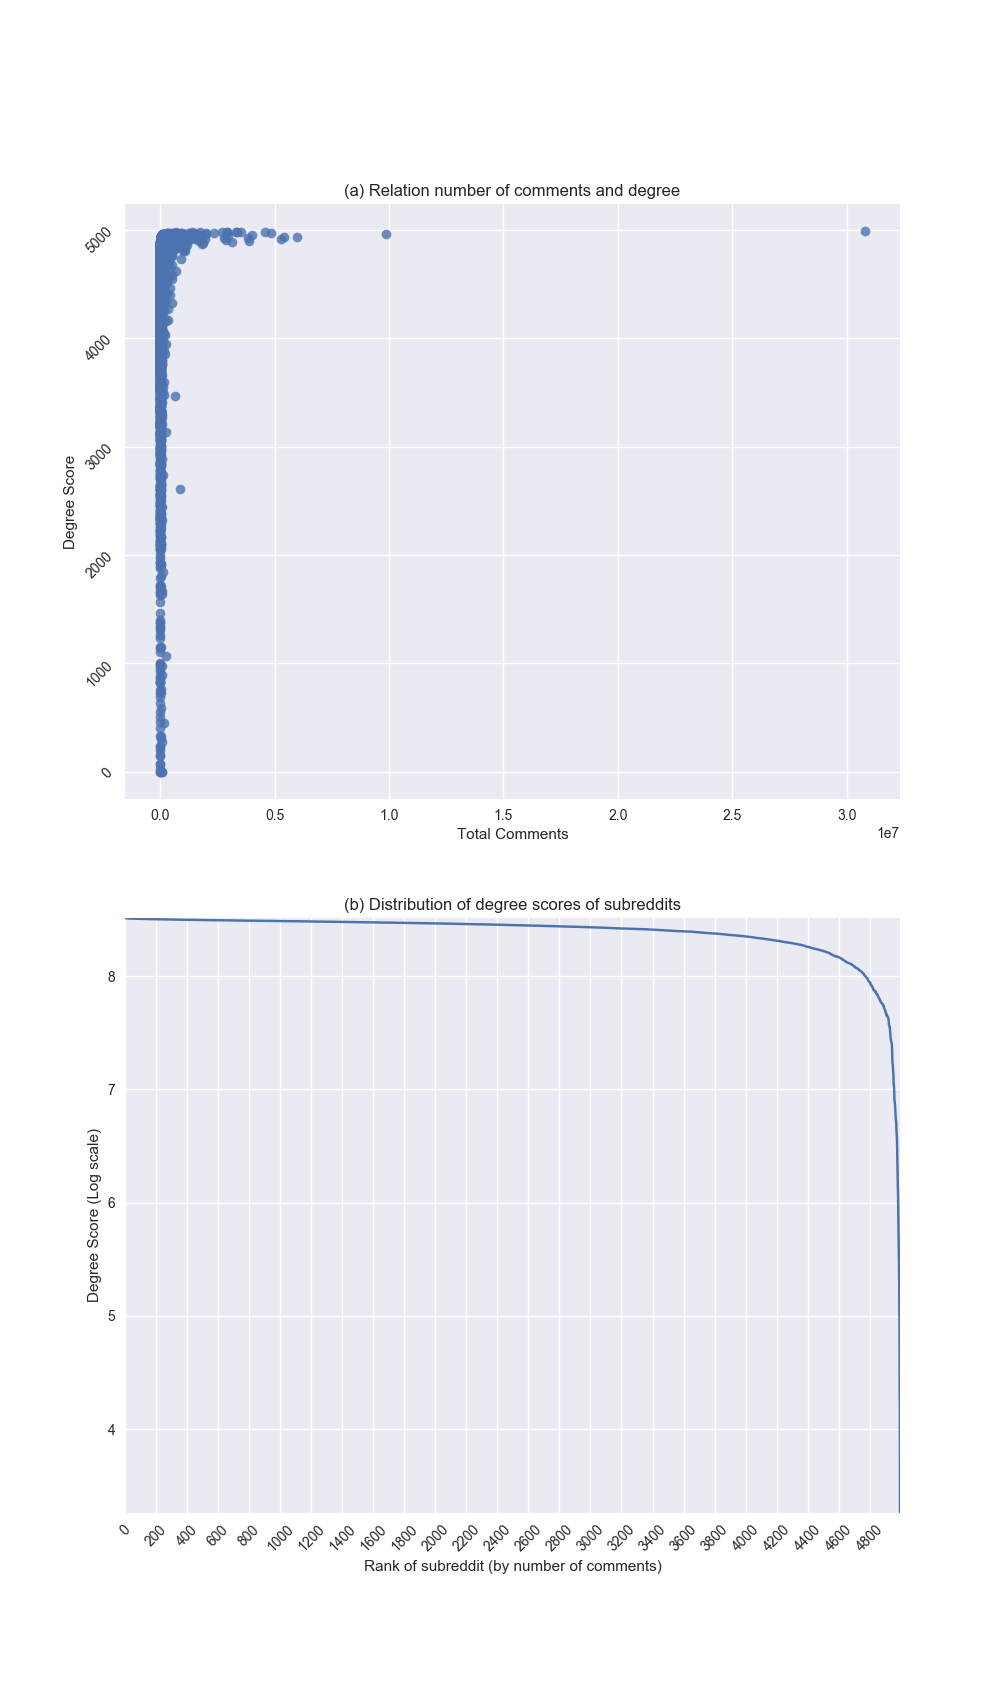
\includegraphics[width=\textwidth]{degree.png}
  	\caption{Results of Degree (with respect to comment count)}
  	\label{fig:degree}
\end{figure}

\begin{figure}[p]
	\centering
  	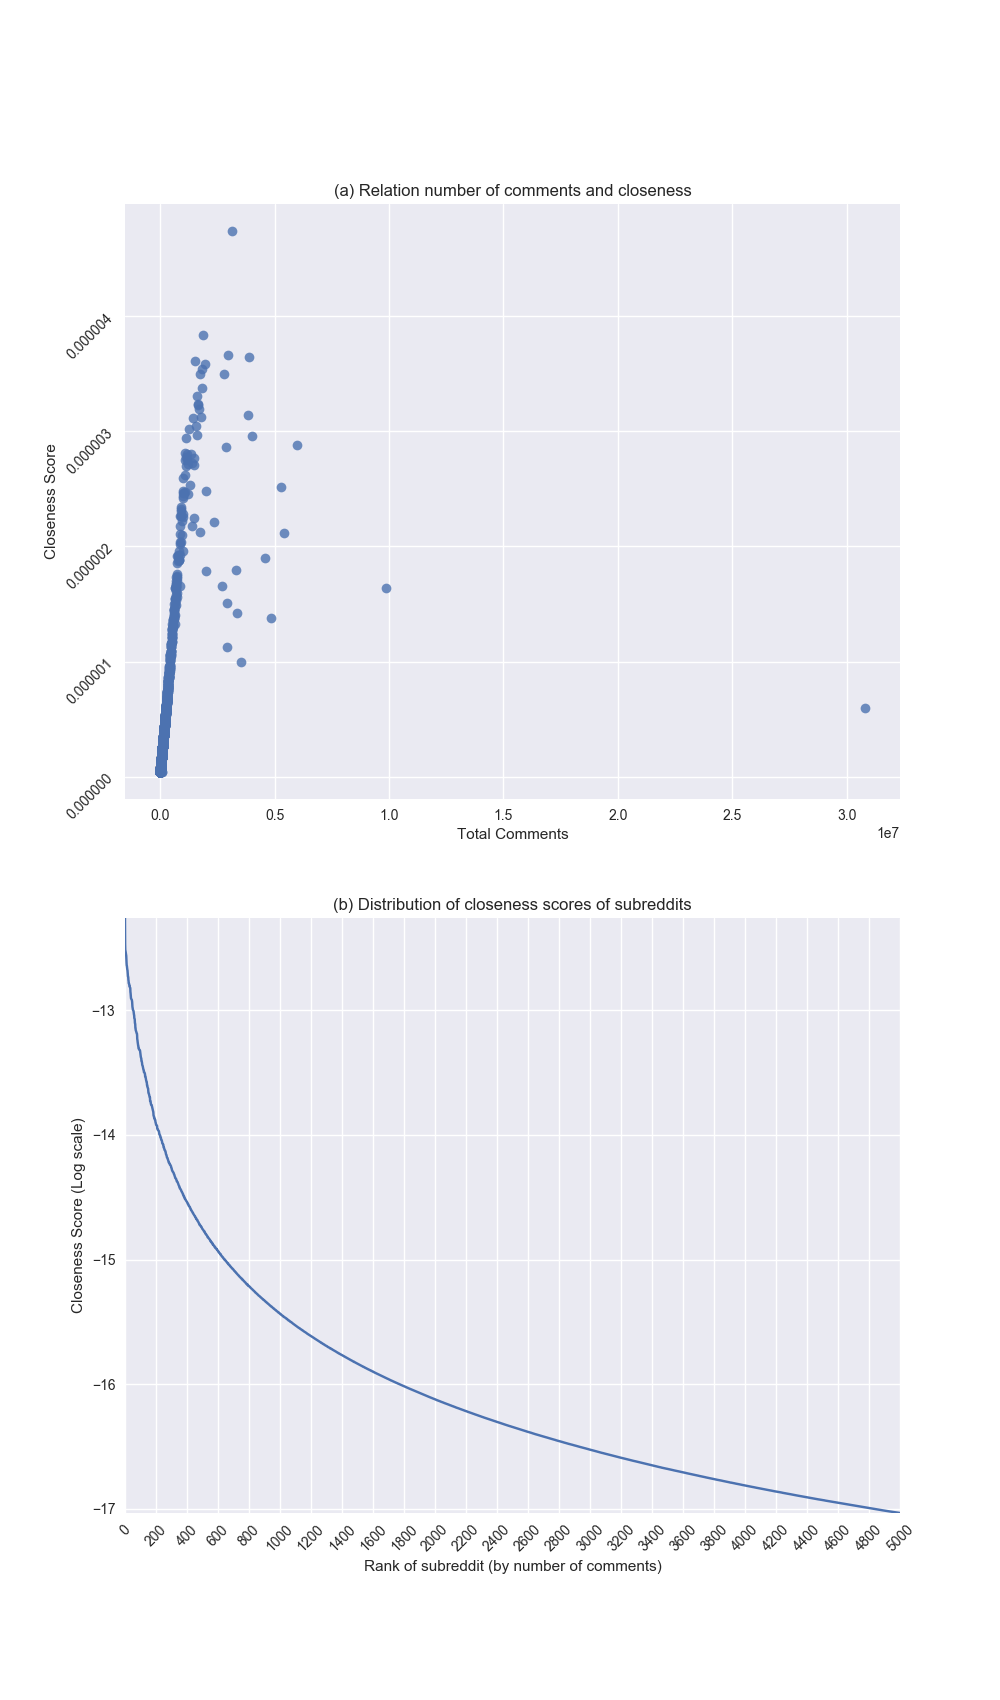
\includegraphics[width=\textwidth]{closeness.png}
  	\caption{Results of Closeness (with respect to comment count)}
  	\label{fig:closeness}
\end{figure}

\begin{figure}[p]
	\centering
  	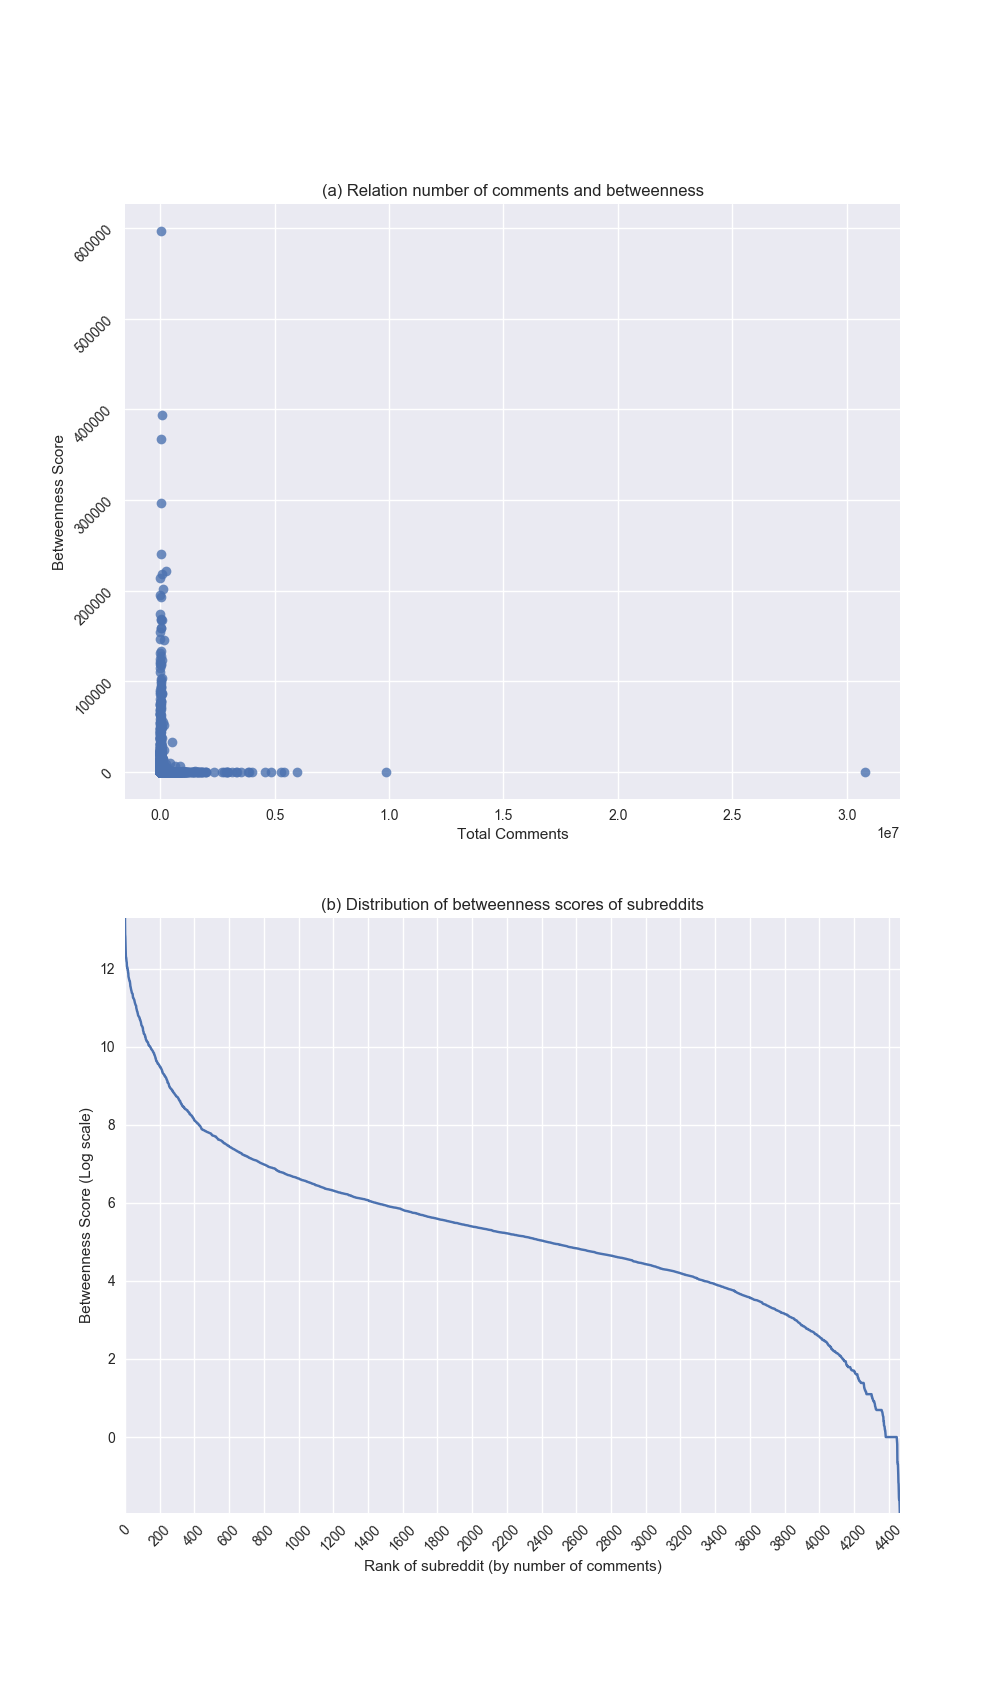
\includegraphics[width=\textwidth]{betweenness.png}
  	\caption{Results of Betweenness (with respect to comment count)}
  	\label{fig:betweenness}
\end{figure}
\begin{figure}[p]
	\centering
  	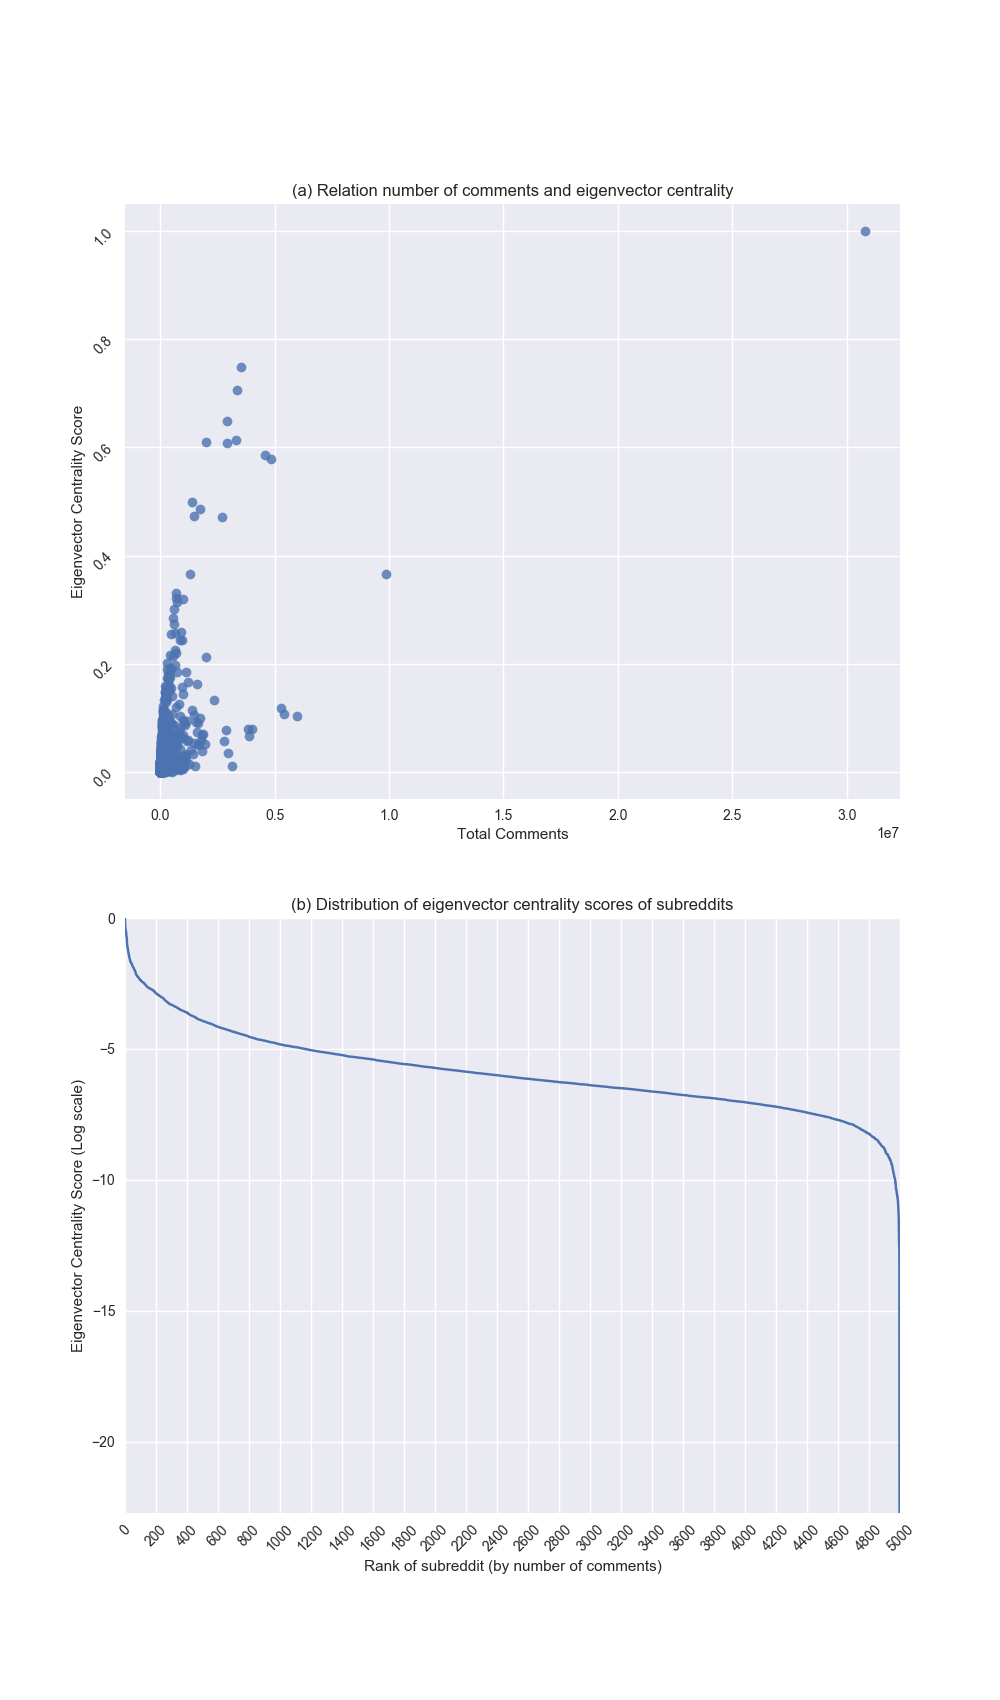
\includegraphics[width=\textwidth]{eigen_centrality.png}
  	\caption{Results of Eigenvector Centrality (with respect to comment count)}
  	\label{fig:eigen_centrality}
\end{figure}

\newpage
\subsection{Regression with all features included}\label{regression-all}

The comment count seems to be significant for some of the centrality measures we adopted, and we managed to obtain very similar results to previous studies, even using a completely different dataset. The next step was to create a linear regression model using features obtained from LIWC. We ran it on our set of 5000 subreddits, from which we extracted 500 comments each: those that were deemed popular by the community (ranked by the highest scores overall, in our given timeframe). This resulted in a feature vector of 93 dimensions, described in section \ref{liwc}, and an additional two: the average number of posts per day, per subreddit (AvgPost), and the average number of unique users who posted in a subreddit per day (AvgAuthor).

Results generated by Jialun Wu \cite{masters}, by running their full regression algorithm are presented below, in table \ref{tab:full-regression-old}. The eigenvector centrality provided the best results, due to the low Residual Standard Error and significantly higher F-ratio than the rest of the measurements. In fact, the Adjusted R-squared measurement is the highest observed such value, meaning that about 80\% of the variance in the eigenvector centrality can be explained with the used feature vector \cite{masters}. 

\begin{table}[!h]
\centering
\resizebox{.9\textwidth}{!}{%
\begin{tabular}{@{}ccccc@{}}
\toprule
                        & Degree & Betweenness & Closeness & Eigenvector    \\ \midrule
Residual Standard Error & 0.69   & 0.80        & 0.85      & \textbf{0.44}  \\
R-squared               & 0.57   & 0.41        & 0.35      & \textbf{0.82}  \\
Adjusted R-squared      & 0.52   & 0.35        & 0.28      & \textbf{0.80}  \\
F-ratio                 & 12.46  & 6.73        & 5.08      & \textbf{43.87} \\ \midrule
Degree of Freedom       & \multicolumn{4}{c}{904}                           \\
P-value                 & \multicolumn{4}{c}{\textless{}0.0001***}          \\ \bottomrule
\end{tabular}%
}
\caption{Results for full regression on the limited dataset}
\label{tab:full-regression-old}
\end{table}

The values in our table (\ref{tab:full-regression-new}) are similar, however, in our case Closeness seems to be a better fit than Betweenness, with degree centrality the best out of the three. However, our eigenvector centrality measure remains the best, with an Adjusted R-squared of 0.77, and increased F-ratio's acrross the board, probably due to the increased dataset.

\begin{table}[!h]
\centering
\resizebox{.9\textwidth}{!}{%
\begin{tabular}{@{}ccccc@{}}
\toprule
                        & Degree & Betweenness & Closeness & Eigenvector     \\ \midrule
Residual Standard Error & 0.77   & 0.90        & 0.85      & \textbf{0.48}   \\
R-squared               & 0.42   & 0.21        & 0.30      & \textbf{0.77}   \\
Adjusted R-squared      & 0.41   & 0.19        & 0.29      & \textbf{0.77}   \\
F-ratio                 & 37.72  & 13.35       & 22.08     & \textbf{175.10} \\ \midrule
Degree of Freedom       & \multicolumn{4}{c}{4904}                           \\
P-value                 & \multicolumn{4}{c}{\textless{}0.0001***}           \\ \bottomrule
\end{tabular}%
}
\caption{Results for full regression of the expanded dataset}
\label{tab:full-regression-new}
\end{table}

\subsection{Regression with significant features}\label{regression-stepwise}

As mention previously, for our second suite of tests, we evaluated multicollinearity between input features and eliminated them on the basis of the variance inflation factor, calculated during our previous round of testing. Each time we ran the tests, we remove the predictor with the largest VIF value, and continued this process until those that were left presented VIF's smaller than our chosen threshold of 10. Afterwards, we ran a stepwise regression, which further reduced the number of statistically significant predictors by using the AIC value as an optimiser.

We present the previously removed predictors by Wu \cite{masters} in table \ref{list:vif-old-rq1}. A total of 29 predictors were removed.

\begin{table}[!h]
\centering
\resizebox{\textwidth}{!}{%
\begin{tabular}{@{}l@{}}
\toprule
AllPunc, pronoun, ppron, affect, function, relativ, Dic, cogproc, Analytic,      \\
informal, social, verb, bio, drives, percept, negemo, Authentic, auxverb, Clout, \\
shehe, differ, prep, AvgAuthor, adverb, Tone, focuspresent, OtherP, conj, adj    \\ \bottomrule
\end{tabular}%
}
\caption{Predictors that were removed in the limited dataset}
\label{list:vif-old-rq1}
\end{table}

The ones we removed in our testing can be found in table \ref{list:vif-new-rq1}. As can be seen our list shrunk by 5 elements, leading to only 24 being removed. Our list contains only a single element which was not removed previously "posemo", which counts words categorised as representing positive emotions, such as "love", "nice", and "sweet".

\begin{table}[!h]
\centering
\resizebox{\textwidth}{!}{%
\begin{tabular}{@{}l@{}}
\toprule
AllPunc, ppron, pronoun, affect, function., informal, Dic, Analytic, \\
cogproc, relativ, social, bio, verb, percept, negemo, drives, shehe, \\
AvgAuthor, Authentic, focuspresent, Clout, posemo, auxverb, prep   \\ \bottomrule
\end{tabular}%
}
\caption{Predictors that were removed in the expanded dataset}
\label{list:vif-new-rq1}
\end{table}

\newpage

The results for the stepwise regression aren't very surprising, but improvement can be noticed in all F-ratio's, except for the eigenvector measure. The model seems to be more confident in the results, since it can better explain the level of improvement of the prediction, compared to the innacuracy. Table \ref{tab:stepwise-old} gives a summary of the results.

\begin{table}[!h]
\centering
\resizebox{\textwidth}{!}{%
\begin{tabular}{@{}ccccc@{}}
\toprule
                        & Degree & Betweenness & Closeness & Eigenvector    \\ \midrule
Residual Standard Error & 0.72   & 0.81        & 0.85      & \textbf{0.69}  \\
R-squared               & 0.50   & 0.36        & 0.29      & \textbf{0.54}  \\
Adjusted R-squared      & 0.48   & 0.34        & 0.27      & \textbf{0.52}  \\
F-ratio                 & 23.47  & 18.81       & 15.02     & \textbf{38.91} \\ \midrule
Degree of Freedom       & 970    & 970         & 971       & 970            \\
P-value                 & \multicolumn{4}{c}{\textless{}0.0001***}          \\ \bottomrule
\end{tabular}%
}
\caption{Stepwise regression results on the limited dataset}
\label{tab:stepwise-old}
\end{table}

In our testing we noticed a similar trend when compared to the full regression model results presented earlier. F-ratio's have improved across the board, with the exception of the eigenvector, which still have the best overall scores, but now the degree centrality measure is a close second. However, it is obvious that the larger dataset provides more confident results, it also seems to have reduced the adjusted R-squared values, meaning that even this full list of predictors is not able to completely, or even in majority, describe the variance seen in the results. 

\begin{table}[!h]
\centering
\resizebox{\textwidth}{!}{%
\begin{tabular}{@{}ccccc@{}}
\toprule
                        & Degree & Betweenness & Closeness & Eigenvector     \\ \midrule
Residual Standard Error & 0.78   & 0.91      & 0.85    & \textbf{0.76} \\
R-squared               & 0.40   & 0.17      & 0.28    & \textbf{0.43} \\
Adjusted R-squared      & 0.40   & 0.16      & 0.27    & \textbf{0.43} \\
F-ratio                 & 66.24  & 21.87     & 56.19   & \textbf{105.50}  \\ \midrule
Degree of Freedom       & 4949   & 4952        & 4965      & 4963            \\
P-value                 & \multicolumn{4}{c}{\textless{}0.0001***}           \\ \bottomrule
\end{tabular}%
}
\caption{Stepwise regression results on the increased dataset}
\label{tab:stepwise-new}
\end{table}

Tables \ref{tab:rq1-betweenness}, \ref{tab:rq1-closeness}, \ref{tab:rq1-degree}, and \ref{tab:rq1-eigen}, give the full list of significant predictors for the stepwise regression model, in each of the four centrality measurement categories.

\newpage

\begin{table}[p]
\centering
\caption{RQ1 betweenness}
\label{tab:rq1-betweenness}
\resizebox{.7\textwidth}{!}{%
\begin{tabular}{rcccr}
\hline
            & Estimate   & Std. Error & t value & Pr(\textgreater{}$\rvert$t$\rvert$) \\ \hline
(Intercept) & 1.220e-16  & 1.293e-02  & 0.000   & 1.000000                            \\
WC          & -2.753e-02 & 1.881e-02  & -1.463  & 0.143423                            \\
Tone        & 4.877e-02  & 2.390e-02  & 2.040   & 0.041373 *                          \\
WPS         & -1.527e-01 & 1.749e-02  & -8.728  & \textless 2e-16 ***                 \\
Sixltr      & 6.182e-02  & 2.092e-02  & 2.955   & 0.003143 **                         \\
we          & -6.759e-02 & 2.311e-02  & -2.924  & 0.003466 **                         \\
you         & -4.352e-02 & 2.012e-02  & -2.163  & 0.030612 *                          \\
ipron       & -1.435e-01 & 2.535e-02  & -5.662  & 1.58e-08 ***                        \\
article     & -5.834e-02 & 1.982e-02  & -2.944  & 0.003257 **                         \\
adverb      & -6.552e-02 & 2.987e-02  & -2.194  & 0.028317 *                          \\
conj        & 1.577e-01  & 3.567e-02  & 4.421   & 1.00e-05 ***                        \\
adj         & -6.026e-02 & 2.841e-02  & -2.121  & 0.033949 *                          \\
compare     & -5.188e-02 & 2.858e-02  & -1.815  & 0.069563 .                          \\
interrog    & -6.923e-02 & 2.505e-02  & -2.763  & 0.005742 **                         \\
number      & 3.497e-02  & 1.604e-02  & 2.181   & 0.029233 *                          \\
quant       & 3.750e-02  & 2.100e-02  & 1.786   & 0.074144 .                          \\
anger       & 6.221e-02  & 2.847e-02  & 2.185   & 0.028944 *                          \\
friend      & -6.369e-02 & 1.787e-02  & -3.565  & 0.000367 ***                        \\
insight     & 1.929e-01  & 2.174e-02  & 8.872   & \textless 2e-16 ***                 \\
discrep     & -6.713e-02 & 2.503e-02  & -2.682  & 0.007339 **                         \\
tentat      & -6.289e-02 & 2.909e-02  & -2.162  & 0.030658 *                          \\
differ      & 1.152e-01  & 3.441e-02  & 3.348   & 0.000819 ***                        \\
body        & 8.011e-02  & 2.126e-02  & 3.768   & 0.000167 ***                        \\
health      & -3.781e-02 & 1.602e-02  & -2.360  & 0.018318 *                          \\
affiliation & 8.287e-02  & 2.589e-02  & 3.202   & 0.001376 **                         \\
achieve     & -4.672e-02 & 2.406e-02  & -1.942  & 0.052184 .                          \\
reward      & 8.912e-02  & 2.298e-02  & 3.877   & 0.000107 ***                        \\
focuspast   & 2.988e-02  & 1.887e-02  & 1.583   & 0.113378                            \\
focusfuture & 4.831e-02  & 2.049e-02  & 2.358   & 0.018428 *                          \\
motion      & 9.404e-02  & 1.685e-02  & 5.581   & 2.51e-08 ***                        \\
work        & -3.957e-02 & 1.932e-02  & -2.048  & 0.040636 *                          \\
leisure     & -5.333e-02 & 1.708e-02  & -3.123  & 0.001800 **                         \\
money       & 5.627e-02  & 1.705e-02  & 3.300   & 0.000974 ***                        \\
relig       & -4.043e-02 & 1.412e-02  & -2.862  & 0.004227 **                         \\
death       & -5.530e-02 & 1.597e-02  & -3.462  & 0.000540 ***                        \\
swear       & -4.010e-02 & 2.531e-02  & -1.584  & 0.113237                            \\
netspeak    & 4.963e-02  & 3.029e-02  & 1.638   & 0.101386                            \\
filler      & 2.446e-02  & 1.420e-02  & 1.722   & 0.085170 .                          \\
Period      & -2.127e-02 & 1.479e-02  & -1.438  & 0.150515                            \\
Comma       & 3.562e-02  & 1.797e-02  & 1.982   & 0.047534 *                          \\
Colon       & -5.882e-02 & 1.707e-02  & -3.446  & 0.000574 ***                        \\
QMark       & 3.756e-02  & 1.777e-02  & 2.114   & 0.034577 *                          \\
Exclam      & 1.903e-02  & 1.334e-02  & 1.426   & 0.153888                            \\
Dash        & 3.003e-02  & 1.688e-02  & 1.779   & 0.075296 .                          \\
Quote       & 1.478e-01  & 1.946e-02  & 7.596   & 3.63e-14 ***                        \\
Apostro     & -7.927e-02 & 2.217e-02  & -3.576  & 0.000353 ***                        \\
Parenth     & -4.608e-02 & 2.649e-02  & -1.740  & 0.081972 .                          \\
OtherP      & 2.767e-01  & 3.184e-02  & 8.690   & \textless 2e-16 ***                 \\ \hline
\multicolumn{5}{c}{Signif. codes:  0 ‘***’ 0.001 ‘**’ 0.01 ‘*’ 0.05 ‘.’ 0.1 ‘ ’ 1}    \\ \hline
\end{tabular}%
}
\end{table}

\begin{table}[p]
\centering
\caption{RQ1 closeness}
\label{tab:rq1-closeness}
\resizebox{.8\textwidth}{!}{%
\begin{tabular}{rcccr}
\hline
            & Estimate   & Std. Error & t value & Pr(\textgreater{}$\rvert$t$\rvert$) \\ \hline
(Intercept) & -1.441e-16 & 1.206e-02  & 0.000   & 1.000000                            \\
AvgPost     & 4.175e-01  & 1.226e-02  & 34.042  & \textless 2e-16 ***                 \\
Tone        & -4.929e-02 & 1.816e-02  & -2.714  & 0.006668 **                         \\
WPS         & -2.284e-02 & 1.418e-02  & -1.611  & 0.107294                            \\
Sixltr      & -4.234e-02 & 1.791e-02  & -2.363  & 0.018154 *                          \\
we          & -6.526e-02 & 2.047e-02  & -3.188  & 0.001439 **                         \\
ipron       & 7.152e-02  & 2.145e-02  & 3.334   & 0.000861 ***                        \\
conj        & -1.632e-01 & 3.104e-02  & -5.258  & 1.52e-07 ***                        \\
negate      & -3.810e-02 & 1.588e-02  & -2.400  & 0.016454 *                          \\
interrog    & 8.642e-02  & 2.139e-02  & 4.040   & 5.44e-05 ***                        \\
number      & -2.113e-02 & 1.466e-02  & -1.441  & 0.149543                            \\
anger       & 7.679e-02  & 2.384e-02  & 3.221   & 0.001287 **                         \\
family      & 3.341e-02  & 1.415e-02  & 2.362   & 0.018224 *                          \\
friend      & 3.336e-02  & 1.565e-02  & 2.131   & 0.033161 *                          \\
discrep     & 3.114e-02  & 2.170e-02  & 1.435   & 0.151333                            \\
tentat      & -7.094e-02 & 2.553e-02  & -2.779  & 0.005478 **                         \\
certain     & 4.331e-02  & 1.750e-02  & 2.475   & 0.013350 *                          \\
differ      & -8.702e-02 & 3.137e-02  & -2.774  & 0.005554 **                         \\
affiliation & 6.437e-02  & 2.190e-02  & 2.939   & 0.003305 **                         \\
power       & 2.656e-02  & 1.581e-02  & 1.680   & 0.093040 .                          \\
focuspast   & -4.028e-02 & 1.750e-02  & -2.301  & 0.021410 *                          \\
focusfuture & 5.729e-02  & 1.977e-02  & 2.899   & 0.003765 **                         \\
space       & -4.775e-02 & 1.647e-02  & -2.900  & 0.003752 **                         \\
time        & 5.919e-02  & 2.023e-02  & 2.925   & 0.003455 **                         \\
money       & 3.514e-02  & 1.372e-02  & 2.561   & 0.010474 *                          \\
swear       & -5.760e-02 & 2.045e-02  & -2.816  & 0.004876 **                         \\
netspeak    & -7.049e-02 & 1.763e-02  & -3.999  & 6.47e-05 ***                        \\
filler      & -3.248e-02 & 1.311e-02  & -2.477  & 0.013290 *                          \\
Period      & -3.996e-02 & 1.352e-02  & -2.956  & 0.003134 **                         \\
Colon       & 7.610e-02  & 1.574e-02  & 4.833   & 1.38e-06 ***                        \\
SemiC       & -1.825e-02 & 1.279e-02  & -1.427  & 0.153608                            \\
QMark       & -7.770e-02 & 1.579e-02  & -4.920  & 8.96e-07 ***                        \\
Dash        & -5.175e-02 & 1.514e-02  & -3.419  & 0.000634 ***                        \\
Quote       & 5.489e-02  & 1.548e-02  & 3.546   & 0.000394 ***                        \\
Apostro     & -3.908e-02 & 1.952e-02  & -2.002  & 0.045294 *                          \\ \hline
\multicolumn{5}{c}{Signif. codes:  0 ‘***’ 0.001 ‘**’ 0.01 ‘*’ 0.05 ‘.’ 0.1 ‘ ’ 1}    \\ \hline
\end{tabular}%
}
\end{table}

\begin{table}[p]
\centering
\caption{RQ1 degree}
\label{tab:rq1-degree}
\resizebox{.7\textwidth}{!}{%
\begin{tabular}{rcccr}
\hline
            & Estimate   & Std. Error & t value & Pr(\textgreater{}$\rvert$t$\rvert$) \\ \hline
(Intercept) & -8.650e-16 & 1.100e-02  & 0.000   & 1.000000                            \\
AvgPost     & 6.135e-02  & 1.117e-02  & 5.491   & 4.20e-08 ***                        \\
WC          & -1.539e-01 & 1.547e-02  & -9.943  & \textless 2e-16 ***                 \\
Tone        & -3.764e-02 & 2.034e-02  & -1.851  & 0.064254 .                          \\
you         & -5.324e-02 & 1.643e-02  & -3.239  & 0.001205 **                         \\
they        & 3.836e-02  & 1.510e-02  & 2.540   & 0.011104 *                          \\
ipron       & 1.622e-01  & 2.313e-02  & 7.012   & 2.67e-12 ***                        \\
article     & 1.220e-01  & 1.815e-02  & 6.722   & 2.00e-11 ***                        \\
adverb      & -4.857e-02 & 2.601e-02  & -1.868  & 0.061876 .                          \\
conj        & -1.357e-01 & 3.145e-02  & -4.316  & 1.62e-05 ***                        \\
negate      & -9.465e-02 & 1.486e-02  & -6.370  & 2.05e-10 ***                        \\
compare     & 7.708e-02  & 1.979e-02  & 3.895   & 9.95e-05 ***                        \\
interrog    & 1.237e-01  & 2.203e-02  & 5.613   & 2.10e-08 ***                        \\
number      & -8.378e-02 & 1.298e-02  & -6.454  & 1.19e-10 ***                        \\
quant       & -9.782e-02 & 1.897e-02  & -5.158  & 2.60e-07 ***                        \\
anger       & 5.265e-02  & 2.287e-02  & 2.302   & 0.021364 *                          \\
sad         & 6.009e-02  & 1.451e-02  & 4.142   & 3.49e-05 ***                        \\
family      & 8.333e-02  & 1.477e-02  & 5.640   & 1.79e-08 ***                        \\
friend      & 1.131e-01  & 1.544e-02  & 7.327   & 2.73e-13 ***                        \\
female      & -7.794e-02 & 1.601e-02  & -4.867  & 1.17e-06 ***                        \\
male        & -2.892e-02 & 1.759e-02  & -1.644  & 0.100342                            \\
insight     & -4.672e-02 & 1.689e-02  & -2.766  & 0.005701 **                         \\
cause       & 3.388e-02  & 1.584e-02  & 2.138   & 0.032551 *                          \\
tentat      & -1.484e-01 & 2.482e-02  & -5.977  & 2.43e-09 ***                        \\
certain     & 5.527e-02  & 1.692e-02  & 3.267   & 0.001093 **                         \\
differ      & 9.390e-02  & 3.033e-02  & 3.096   & 0.001972 **                         \\
feel        & 2.836e-02  & 1.602e-02  & 1.771   & 0.076700 .                          \\
body        & 3.482e-02  & 1.964e-02  & 1.773   & 0.076331 .                          \\
sexual      & -4.400e-02 & 2.048e-02  & -2.148  & 0.031723 *                          \\
ingest      & 3.723e-02  & 1.245e-02  & 2.991   & 0.002795 **                         \\
affiliation & -7.100e-02 & 1.564e-02  & -4.540  & 5.75e-06 ***                        \\
achieve     & 1.013e-01  & 2.044e-02  & 4.954   & 7.52e-07 ***                        \\
power       & -6.668e-02 & 1.749e-02  & -3.812  & 0.000140 ***                        \\
reward      & -8.658e-02 & 1.949e-02  & -4.442  & 9.11e-06 ***                        \\
risk        & -5.460e-02 & 1.674e-02  & -3.262  & 0.001114 **                         \\
focuspast   & -5.369e-02 & 1.686e-02  & -3.184  & 0.001461 **                         \\
motion      & -5.472e-02 & 1.496e-02  & -3.657  & 0.000258 ***                        \\
space       & 4.053e-02  & 1.918e-02  & 2.113   & 0.034668 *                          \\
leisure     & 6.780e-02  & 1.414e-02  & 4.796   & 1.66e-06 ***                        \\
home        & 3.972e-02  & 1.343e-02  & 2.958   & 0.003112 **                         \\
relig       & 2.743e-02  & 1.210e-02  & 2.267   & 0.023452 *                          \\
death       & 2.925e-02  & 1.335e-02  & 2.191   & 0.028468 *                          \\
netspeak    & -1.822e-01 & 2.514e-02  & -7.249  & 4.85e-13 ***                        \\
assent      & -3.797e-02 & 1.191e-02  & -3.189  & 0.001438 **                         \\
nonflu      & -4.565e-02 & 1.339e-02  & -3.409  & 0.000657 ***                        \\
QMark       & -7.712e-02 & 1.516e-02  & -5.086  & 3.78e-07 ***                        \\
Exclam      & -3.062e-02 & 1.138e-02  & -2.691  & 0.007154 **                         \\
Dash        & 5.770e-02  & 1.277e-02  & 4.519   & 6.36e-06 ***                        \\
Quote       & -1.470e-01 & 1.384e-02  & -10.623 & \textless 2e-16 ***                 \\
Apostro     & 8.640e-02  & 1.918e-02  & 4.505   & 6.79e-06 ***                        \\
OtherP      & -9.540e-02 & 2.409e-02  & -3.960  & 7.61e-05 ***                        \\ \hline
\multicolumn{5}{c}{Signif. codes:  0 ‘***’ 0.001 ‘**’ 0.01 ‘*’ 0.05 ‘.’ 0.1 ‘ ’ 1}    \\ \hline
\end{tabular}%
}
\end{table}

\begin{table}[p]
\centering
\caption{RQ1 eigen}
\label{tab:rq1-eigen}
\resizebox{.8\textwidth}{!}{%
\begin{tabular}{rlccl}
\hline
            & \multicolumn{1}{c}{Estimate} & Std. Error & t value & Pr(\textgreater{}$\rvert$t$\rvert$) \\ \hline
(Intercept) & -1.309e-16                   & 1.068e-02  & 0.000   & 1.000000                            \\
AvgPost     & 5.779e-01                    & 1.086e-02  & 53.225  & \textless 2e-16 ***                 \\
WC          & -2.524e-02                   & 1.407e-02  & -1.795  & 0.072767 .                          \\
Sixltr      & -2.363e-02                   & 1.563e-02  & -1.512  & 0.130579                            \\
i           & 4.266e-02                    & 1.761e-02  & 2.422   & 0.015462 *                          \\
you         & 2.227e-02                    & 1.508e-02  & 1.477   & 0.139793                            \\
they        & 2.144e-02                    & 1.417e-02  & 1.514   & 0.130188                            \\
ipron       & 9.789e-02                    & 2.111e-02  & 4.636   & 3.64e-06 ***                        \\
article     & 7.598e-02                    & 1.580e-02  & 4.810   & 1.56e-06 ***                        \\
conj        & -8.698e-02                   & 2.981e-02  & -2.918  & 0.003535 **                         \\
negate      & -2.898e-02                   & 1.410e-02  & -2.055  & 0.039895 *                          \\
adj         & -6.898e-02                   & 2.140e-02  & -3.223  & 0.001275 **                         \\
compare     & 9.538e-02                    & 2.260e-02  & 4.220   & 2.49e-05 ***                        \\
interrog    & 5.723e-02                    & 1.965e-02  & 2.913   & 0.003601 **                         \\
quant       & -3.486e-02                   & 1.705e-02  & -2.045  & 0.040946 *                          \\
family      & 7.280e-02                    & 1.318e-02  & 5.522   & 3.53e-08 ***                        \\
friend      & 6.618e-02                    & 1.435e-02  & 4.612   & 4.09e-06 ***                        \\
male        & 3.213e-02                    & 1.735e-02  & 1.852   & 0.064140 .                          \\
cause       & 2.628e-02                    & 1.515e-02  & 1.734   & 0.082906 .                          \\
differ      & -1.177e-01                   & 2.858e-02  & -4.119  & 3.87e-05 ***                        \\
hear        & -2.732e-02                   & 1.258e-02  & -2.171  & 0.029978 *                          \\
body        & 4.272e-02                    & 1.648e-02  & 2.592   & 0.009576 **                         \\
ingest      & 4.760e-02                    & 1.162e-02  & 4.096   & 4.27e-05 ***                        \\
affiliation & -4.148e-02                   & 1.484e-02  & -2.796  & 0.005190 **                         \\
achieve     & -5.682e-02                   & 1.699e-02  & -3.345  & 0.000830 ***                        \\
focuspast   & 4.198e-02                    & 1.609e-02  & 2.610   & 0.009095 **                         \\
focusfuture & -3.018e-02                   & 1.500e-02  & -2.012  & 0.044279 *                          \\
work        & 8.155e-02                    & 1.416e-02  & 5.758   & 9.04e-09 ***                        \\
leisure     & 5.461e-02                    & 1.395e-02  & 3.914   & 9.21e-05 ***                        \\
death       & 2.121e-02                    & 1.195e-02  & 1.774   & 0.076072 .                          \\
swear       & -4.765e-02                   & 1.442e-02  & -3.305  & 0.000955 ***                        \\
netspeak    & -5.102e-02                   & 1.746e-02  & -2.921  & 0.003502 **                         \\
Colon       & 5.040e-02                    & 1.374e-02  & 3.669   & 0.000246 ***                        \\
QMark       & -3.789e-02                   & 1.378e-02  & -2.750  & 0.005981 **                         \\
Dash        & -2.768e-02                   & 1.362e-02  & -2.032  & 0.042247 *                          \\
Apostro     & -6.025e-02                   & 1.829e-02  & -3.294  & 0.000996 ***                        \\
tentat      & 3.293e-02                    & 2.281e-02  & 1.444   & 0.148792                            \\ \hline
\multicolumn{5}{c}{Signif. codes:  0 ‘***’ 0.001 ‘**’ 0.01 ‘*’ 0.05 ‘.’ 0.1 ‘ ’ 1}                      \\ \hline
\end{tabular}%
}
\end{table}


\chapter{Research Objective 2: Reddit-specific features analysis}\label{reddit-features-results}

\section{Overview of Research Objective 2}

For our second research objective, we included all the features that could be mined from the metadata present in the increased dataset on Google BigQuery. As such, we intially included AvgPost and AvgAuthor, however, since we used these measures to build others, such as AvgPostsPerAuthor, and TotalGoldPerAvgAuthor, these predictors had a high multicollinearity with each other. The VIF revealed this, and we removed them by using the same process as in our first research objective. Although we initially started out by analysing all of the 15 predictors, it quickly became apparent that the stepwise regression model would more be suitable for this task, due to the similarity present in many of the factors we chose. Table \ref{list:vif-new-rq2} presents 9 out of the 15 that were removed.

\begin{table}[!h]
\centering
\resizebox{\textwidth}{!}{%
\begin{tabular}{@{}|l|@{}}
\toprule
ScoreOver200Count, ScoreOver1000Count, AvgScorePerDay, ScoreOver100Count,  \\
ScoreOver500Count, AvgGildedPostsPerDay, AvgAuthor, AvgPost, AvgGoldPerDay \\ \bottomrule
\end{tabular}%
}
\caption{Predictors that were removed for the additional features}
\label{list:vif-new-rq2}
\end{table}

Descriptions for these predictors can be found in section \ref{features} of the Methodology. The choice of different cut-off points for measuring the number of comments above a score, meant that a significant number of these had very similar results, leading to high multicollinearity. Of note is that the two extremes, namely karma scores above 50 (the lowest we measured), and karma scores above 2000 (the highest), were both very significant predictors, except for betweenness centrality, and had a low VIF score. This may lead us to conclude that both are necessary in order to gain a better understanding of how Reddit works in the high-, and tail-end of the distribution of subreddits by popularity.

\newpage

\section{Stepwise Regression Results}

The F-ratio for the Closeness and Eigenvector values in this test reveals that with these predictors, the model presents confidence in the results. The R-squared value of the Eigenvector centrality measurement is able to explain 50\% of the variance with the variance in the remaining 6 predictors, which is an increase on our results which included the content analysis results provided by LIWC.

\begin{table}[!h]
\centering
\resizebox{\textwidth}{!}{%
\begin{tabular}{@{}ccccc@{}}
\toprule
                        & Degree & Betweenness & Closeness & Eigenvector     \\ \midrule
Residual Standard Error & 1.00   & 0.98        & 0.77     & \textbf{0.71}  \\
R-squared               & 0.03   & 0.03        & 0.41    & \textbf{0.50} \\
Adjusted R-squared      & 0.03   & 0.03        & 0.41    & \textbf{0.50} \\
F-ratio                 & 31.90  & 33.23       & 567.70     & \textbf{986.90}  \\ \midrule
Degree of Freedom       & 4979   & 4979        & 4978      & 4979            \\
P-value                 & \multicolumn{4}{c}{\textless{}0.0001***}           \\ \bottomrule
\end{tabular}%
}
\caption{Summary of stepwise regression results for RQ2}
\label{tab:stepwise-rq2}
\end{table}

Tables \ref{tab:rq1-betweenness}, \ref{tab:rq1-closeness}, \ref{tab:rq1-degree}, and \ref{tab:rq1-eigen}, give the full list of significant predictors for the stepwise regression model, in each of the four centrality measurement categories.

\newpage

\begin{table}[]
\centering
\caption{RQ2 betweenness}
\label{tab:rq2-betweenness}
\begin{tabular}{rcccr}
\hline
                      & Estimate  & Std. Error     & t value & Pr(\textgreater{}$\rvert$t$\rvert$) \\ \hline
(Intercept)           & -1.246e-17    & 1.394e-02 & 0.000   & 1.0000                              \\
AvgPostsPerAuthor     & 1.731e-01     & 1.395e-02 & 12.411  & \textless{}2e-16 ***                \\
ScoreOver2000Count    & 3.913e-02     & 2.651e-02 & 1.476   & 0.1400                              \\
ScoreOver50Count      & -5.342e-02    & 2.652e-02 & -2.015  & 0.0440 *                            \\
TotalGoldPerAvgAuthor & 3.533e-02     & 2.423e-02 & 1.458   & 0.1449                              \\
TotalGoldPerAvgPost   & -5.381e-02    & 2.423e-02 & -2.221  & 0.0264 *                            \\ \hline
\multicolumn{5}{c}{Signif. codes:  0 ‘***’ 0.001 ‘**’ 0.01 ‘*’ 0.05 ‘.’ 0.1 ‘ ’ 1}                \\ \hline
\end{tabular}
\end{table}

\begin{table}[]
\centering
\caption{RQ2 closeness}
\label{tab:rq2-closeness}
\begin{tabular}{rcccr}
\hline
                      & Estimate   & Std. Error & t value & Pr(\textgreater{}$\rvert$t$\rvert$) \\ \hline
(Intercept)           & 3.429e-17  & 1.092e-02  & 0.000   & 1.00000                             \\
AvgControversiality   & 3.037e-01  & 2.160e-02  & 14.058  & \textless 2e-16 ***                 \\
AvgPostsPerAuthor     & 4.430e-02  & 1.093e-02  & 4.054   & 5.12e-05 ***                        \\
ScoreOver2000Count    & -7.550e-01 & 2.261e-02  & -33.399 & \textless 2e-16 ***                 \\
ScoreOver50Count      & 7.932e-01  & 3.299e-02  & 24.043  & \textless 2e-16 ***                 \\
TotalGoldPerAvgAuthor & 5.687e-02  & 1.899e-02  & 2.995   & 0.00276 **                          \\
TotalGoldPerAvgPost   & -3.516e-02 & 1.898e-02  & -1.852  & 0.06412 .                           \\ \hline
\multicolumn{5}{c}{Signif. codes:  0 ‘***’ 0.001 ‘**’ 0.01 ‘*’ 0.05 ‘.’ 0.1 ‘ ’ 1}              \\ \hline
\end{tabular}
\end{table}

\begin{table}[]
\centering
\caption{RQ2 degree}
\label{tab:rq2-degree}
\begin{tabular}{rcccr}
\hline
                    & Estimate   & Std. Error & t value & Pr(\textgreater{}$\rvert$t$\rvert$) \\ \hline
(Intercept)         & -6.003e-17 & 1.395e-02  & 0.000   & 1.000000                            \\
AvgControversiality & 4.873e-02  & 2.759e-02  & 1.766   & 0.077406 .                          \\
AvgPostsPerAuthor   & -1.097e-01 & 1.395e-02  & -7.863  & 4.57e-15 ***                        \\
ScoreOver2000Count  & -1.351e-01 & 2.888e-02  & -4.677  & 2.98e-06 ***                        \\
ScoreOver50Count    & 1.604e-01  & 4.214e-02  & 3.806   & 0.000143 ***                        \\
TotalGoldPerAvgPost & 5.894e-02  & 1.396e-02  & 4.222   & 2.47e-05 ***                        \\ \hline
\multicolumn{5}{c}{Signif. codes:  0 ‘***’ 0.001 ‘**’ 0.01 ‘*’ 0.05 ‘.’ 0.1 ‘ ’ 1}            \\ \hline
\end{tabular}
\end{table}

\begin{table}[]
\centering
\caption{RQ2 eigen}
\label{tab:rq2-eigen}
\begin{tabular}{rcccr}
\hline
                      & Estimate   & Std. Error & t value & Pr(\textgreater{}$\rvert$t$\rvert$) \\ \hline
(Intercept)           & -3.035e-17 & 1.004e-02  & 0.000   & 1.000000                            \\
AvgControversiality   & 4.838e-01  & 1.987e-02  & 24.355  & \textless 2e-16 ***                 \\
ScoreOver2000Count    & 1.561e-01  & 2.079e-02  & 7.509   & 7.02e-14 ***                        \\
ScoreOver50Count      & 1.185e-01  & 3.034e-02  & 3.905   & 9.55e-05 ***                        \\
TotalGoldPerAvgAuthor & -5.942e-02 & 1.745e-02  & -3.405  & 0.000667 ***                        \\
TotalGoldPerAvgPost   & 1.165e-01  & 1.745e-02  & 6.679   & 2.67e-11 ***                        \\ \hline
\multicolumn{5}{c}{Signif. codes:  0 ‘***’ 0.001 ‘**’ 0.01 ‘*’ 0.05 ‘.’ 0.1 ‘ ’ 1}              \\ \hline
\end{tabular}
\end{table}


\chapter{Research Objective 3: Sentiment, Personality and Engagement analysis of Reddit comments}\label{content-analysis-results}

\section{}

For our final research objective, we used the \textit{"indico.io"} API to generate sentiment, personality and engagement measures for the 5,000 subreddits we chose to include in our study. When fitting our regression model

\begin{table}[!h]
\centering
\resizebox{\textwidth}{!}{%
\begin{tabular}{@{}ccccc@{}}
\toprule
                        & Degree          & Betweenness & Closeness & Eigenvector \\ \midrule
Residual Standard Error & \textbf{0.88}   & 0.96        & 0.99      & 1.00        \\
R-squared               & \textbf{0.23}   & 0.08        & 0.03      & 0.01        \\
Adjusted R-squared      & \textbf{0.23}   & 0.08        & 0.03      & 0.01        \\
F-ratio                 & \textbf{214.00} & 76.88       & 27.95     & 9.78        \\ \midrule
Degree of Freedom       & 4992            & 4993        & 4994      & 4995        \\
P-value                 & \multicolumn{4}{c}{\textless{}0.0001***}                \\ \bottomrule
\end{tabular}%
}
\caption{Summary of stepwise regression results for RQ3}
\label{tab:stepwise-rq3}
\end{table}

\newpage

\begin{table}[]
\centering
\caption{RQ3 betweenness}
\begin{tabular}{rcccr}
\hline
                    & Estimate & Std. Error     & t value & Pr(\textgreater{}$\rvert$t$\rvert$) \\ \hline
(Intercept)         & -1.369e-16    & 1.354e-02 & 0.000   & 1.0000                              \\
sentiment           & -3.296e-02    & 1.482e-02 & -2.224  & 0.0262 *                            \\
joy                 & 6.333e-02     & 1.602e-02 & 3.953   & 7.82e-05 ***                        \\
surprise            & -2.762e-02    & 1.572e-02 & -1.757  & 0.0789 .                            \\
extraversion        & -8.704e-02    & 2.213e-02 & -3.933  & 8.50e-05 ***                        \\
agreeableness       & 9.101e-02     & 2.279e-02 & 3.994   & 6.59e-05 ***                        \\
twitter\_engagement & -2.526e-01    & 1.453e-02 & -17.379 & \textless 2e-16 ***                 \\ \hline
\multicolumn{5}{c}{Signif. codes: 0 ‘***’ 0.001 ‘**’ 0.01 ‘*’ 0.05 ‘.’ 0.1 ‘ ’ 1}               \\ \hline
\end{tabular}
\end{table}

\begin{table}[]
\centering
\caption{RQ3 closeness}
\begin{tabular}{rcccr}
\hline
                    & Estimate & Std. Error     & t value & Pr(\textgreater{}$\rvert$t$\rvert$) \\ \hline
(Intercept)         & -1.280e-16    & 1.396e-02 & 0.000   & 1                                   \\
sentiment           & -6.589e-02    & 1.498e-02 & -4.400  & 1.11e-05 ***                        \\
openness            & -1.206e-01    & 1.611e-02 & -7.489  & 8.18e-14 ***                        \\
agreeableness       & -7.536e-02    & 1.729e-02 & -4.358  & 1.34e-05 ***                        \\
conscientiousness   & -1.183e-01    & 1.648e-02 & -7.180  & 8.00e-13 ***                        \\
twitter\_engagement & 8.643e-02     & 1.453e-02 & 5.947   & 2.91e-09 ***                        \\ \hline
\multicolumn{5}{c}{Signif. codes:  0 ‘***’ 0.001 ‘**’ 0.01 ‘*’ 0.05 ‘.’ 0.1 ‘ ’ 1}              \\ \hline
\end{tabular}
\end{table}

\begin{table}[]
\centering
\caption{RQ3 degree}
\begin{tabular}{rcccr}
\hline
                    & Estimate  & Std. Error     & t value & Pr(\textgreater{}$\rvert$t$\rvert$) \\ \hline
(Intercept)         & -3.899e-16    & 1.241e-02 & 0.000   & 1.000000                            \\
joy                 & -5.351e-02    & 1.463e-02 & -3.658  & 0.000256 ***                        \\
sadness             & -3.547e-02    & 1.269e-02 & -2.795  & 0.005210 **                         \\
surprise            & 2.203e-02     & 1.449e-02 & 1.520   & 0.128611                            \\
openness            & -2.852e-02    & 1.440e-02 & -1.981  & 0.047693 *                          \\
agreeableness       & -6.415e-02    & 1.456e-02 & -4.406  & 1.07e-05 ***                        \\
conscientiousness   & -7.870e-02    & 1.462e-02 & -5.382  & 7.68e-08 ***                        \\
twitter\_engagement & 4.515e-01     & 1.322e-02 & 34.145  & \textless 2e-16 ***                 \\ \hline
\multicolumn{5}{c}{Signif. codes:  0 ‘***’ 0.001 ‘**’ 0.01 ‘*’ 0.05 ‘.’ 0.1 ‘ ’ 1}              \\ \hline
\end{tabular}
\end{table}

\begin{table}[]
\centering
\caption{RQ3 eigen}
\begin{tabular}{rcccr}
\hline
                    & Estimate  & Std. Error     & t value & Pr(\textgreater{}$\rvert$t$\rvert$) \\ \hline
(Intercept)         & 6.412e-17     & 1.409e-02 & 0.000   & 1.00000                             \\
joy                 & -2.681e-02    & 1.656e-02 & -1.619  & 0.10548                             \\
surprise            & 4.684e-02     & 1.634e-02 & 2.867   & 0.00416 **                          \\
agreeableness       & 3.216e-02     & 1.414e-02 & 2.274   & 0.02301 *                           \\
twitter\_engagement & 6.757e-02     & 1.436e-02 & 4.705   & 2.61e-06 ***                        \\ \hline
\multicolumn{5}{c}{Signif. codes:  0 ‘***’ 0.001 ‘**’ 0.01 ‘*’ 0.05 ‘.’ 0.1 ‘ ’ 1}              \\ \hline
\end{tabular}
\end{table}

\chapter{Discussion}\label{discussion}

\section{Research Objective 1:}\label{rq1}

\section{Research Objective 2:}\label{rq2}

\section{Research Objective 3:}\label{rq3}

\section{Further Work and Limitations}\label{further-work}

%TODO: limitations of centrality measures, topical clustering of subreddits, and there was also something about hierarchical comment analysis in one of the papers

%TODO: talk about density (which is another aspect of SNA)
%TODO: talk about other types of centrality measures, which were not used (and why) - maybe add this to the limitations?

\chapter{Conclusion}\label{conclusion}

%TODO: Talk how the conclusion relates to the background

%TODO: Dunbar's number (https://en.wikipedia.org/wiki/Dunbar%27s_number) 

%TODO: Maybe talk about this a bit? https://www.ben-evans.com/benedictevans/2018/4/2/the-death-of-the-newsfeed
% HN Story for the above: https://news.ycombinator.com/item?id=16741237

\nocite{*}

\bibliographystyle{apalike}
\bibliography{report}

\end{document}
